\chapter*{Introduction}

\reversemarginpar
This essay brings to bear observations of the \acrlong{NEC} (see \citealt{Croft1991}, \citealt{Veselinova2013,Veselinova2016}, \citealt{Hamari} (eds.)) in the context of the Aboriginal languages of Australia. The Australian language ecology is a fertile area for comparative typological work, given its striking linguistic diversity and small, non-sedentary, frequently exogamous populations \citep{Bowern2010}. Some 90\% ($\mathnormal{N\approx290}$) of the languages spoken on the Australian mainland have been reconstructed to the Pama-Nyungan family \citep[see also ][]{OVV1966,Wurm1972,Bowern2012b}, with a common ancestor spoken in Northern Australia almost 6,000 years before present \citep{Bouckaert2018}.

%In view of this linguistic diversity and recent advancements in understanding subgrouping and speciation relations in the family, Pama-Nyungan provides an opportunity to better understand patterns of typological change. 
Taking the negative domains of three Pama-Nyungan subgroups as an empirical testing ground, this chapter describes the relationship between so-called `standard' (\acrshort{sn}) and `existential' negation in an investigation of predictions made by a postulated cyclic change: \acrfull{NEC}.


Represented in figure \ref{fig:croftcycle} The \acrshort{NEC} involves the emergence of explicit markers of existential negation\footnote{
	For the purposes of this paper, similarly to others in the current volume, ``existential negation'' is understood as a linguistic strategy for predicating the \textit{absence} of some entity at a certain location (adapting from Criessels' \citeyearpar[2]{Creissels2014} typology of existential constructions and consonant with the approach taken in \citealp[139]{Veselinova2013}.) Defining `existential predication', McNally also points out the relevance of ``noncanonical sentence types'', distinguished syntactically or lexically, which serve to `introduce the presence or existence of some individual(s)' \citeyearpar[210]{McNally2016}. See also \citealt{Freeze1992} for an analysis that explicitly relates existential to \textsc{locative} and \textsc{possessive} predications.}
  (stage $\mathbb{A\to B}$), which subsequently encroach into the semantic domain of an erstwhile general negative marker (stage $\mathbb{B\to C}$), and finally displace the latter, becoming a standard negation marker without the formal or functional features of an existential negator (stage $\mathbb{C\to A}$). Examples of each of the \acrshort{NEC}'s stages are reproduced in (\nextx) below (these data cited in \citealp[7--12]{Croft1991})
  


%\begin{wrapfigure}{r}{.595\textwidth}
\begin{figure}[h]	\centering
	\begin{tikzpicture}[scale=0.25]\footnotesize
		\tikzstyle{every node}+=[inner sep=0pt]
		\draw [black] (23.6,-7.9) circle (3);
		\draw (23.6,-7.9) node[rectangle split,rectangle split parts=2] {$ \boldsymbol{\mathbb{A}} $\nodepart{second} $\neg\phi/\neg\exists x$};
		\draw [black] (13.2,-24) circle (3);
		\draw (13.2,-24) node[rectangle split,rectangle split parts=2] {$ \boldsymbol{\mathbb{C}} $\nodepart{second} $\nexists\phi/\nexists x$};
		\draw [black] (33.6,-24) circle (3);
		\draw (33.6,-24) node[rectangle split,rectangle split parts=2] {$ \boldsymbol{\mathbb{B}} $\nodepart{second} $\neg\phi/\nexists x$};
		\draw [black] (26.574,-8.22) arc (76.02264:-12.33232:10.957);
		\fill [black] (34.63,-21.19) -- (35.29,-20.52) -- (34.31,-20.3);
		\draw [black] (12.391,-21.12) arc (-171.74775:-253.97416:11.563);
		\fill [black] (20.64,-8.35) -- (19.74,-8.09) -- (20.01,-9.05);
		\draw [black] (31.586,-26.214) arc (-49.16439:-130.83561:12.519);
		\fill [black] (15.21,-26.21) -- (15.49,-27.12) -- (16.15,-26.36);
	\end{tikzpicture}
	
	\caption[The Negative Existential Cycle]{The `Negative Existential cycle' --- a typology (and proposed grammaticalisation trajectory) of standard \& existential negation according to the analyticity of these markers (\citealt{Croft1991}, see also \citealt{Veselinova2016}.) Standard negators $\boldsymbol\neg$ are used to negate both verbal $\phi$ and existential $\boldsymbol{\exists x}$ predicates in stage $ \mathbb{A} $, a suppletive `negative existential' $\nexists$ arises in stage $ \mathbb{B} $ and this marker comes to mark standard negation in stage $ \mathbb{C}$. `Transitional' stages are assumed to occur between each of the labelled stages.}\label{fig:croftcycle}
\end{figure}


\pex\rightcomment{\textbf{Lahu} [\gls{lhu}]} \textsb{Stage $ \mathbb A$: analytic negative existential predication}
\a\begingl\gla šɔ̀-pɔ̄ \textbf{mâ} qay//
\glb tomorrow \textsc{\textbf{neg}} go//
\glft`I'm not going tomorrow'\trailingcitation{\citep[269]{Matisoff1973}}//\endgl
\a\begingl\gla ɔ̀-yâ \textbf{mâ} \textbf{cɔ̀} sɔ̄//
\glb time \textsc{\textbf{neg}} \textsc{\textbf{ex}} \textsc{dur}//
\glft`There's still no time.'\trailingcitation{\citep[339]{Matisoff1973}}//\endgl
\xe

\pex~\rightcomment{\textbf{Amharic} [\gls{amh}]} \textsb{Stage $ \mathbb B $: negative existential predicate (\textit{yälläm} `\gls{negex}')}
\a\begingl\gla \textbf{a}-ysǝbr-\textbf{ɨm}//
\glb\textbf{\gls{neg}}-pass.3ms.\gls{impf}-\gls{neg}//
\glft`He doesn't/won't break.'\trailingcitation{\citep[303]{Leslau1995}}//\endgl
\a\begingl%\gla እንጀራ የለም//
\gla ɨnjǝra \textbf{yǝllǝmm}//
\glc bread \textsc{\textbf{negex}}.3s//
\glft`There's no bread.'\trailingcitation{\citep[715]{Leslau1995}}//\endgl
\xe

\pex~\rightcomment{\textbf{Manam} [\gls{mva}]} \textsb{Stage $ \mathbb C $: homonymous \acrshort{sn} and \gls{negex} (\textit{tágo})}
\a\begingl\gla \textbf{tágo} u-lóŋo//
\glb \textsc{\textbf{neg}(ex)} 1s.\textsc{rl}-hear//
\glft`I did not hear.'\trailingcitation{\citep[385]{Lichtenberk}}//\endgl
\a\begingl\gla anúa-lo tamóata \textbf{tágo} (*i-sóaˀi)//
\glb village-in person \textsc{\textbf{negex}} (*3s.\textsc{rl\textbf{-ex}})//
\glft`There's noone in the village.'  \trailingcitation{\citep[499]{Lichtenberk1983}}//\endgl
\xe

\pex~\begingl\glpreamble\textsb{Stage $ \mathbb{A'} $: emergence of an existential predicate \textit{āhe} optionally disambiguates standard and existential negation}//
\gla \rightcomment{\textbf{Marathi} [\gls{mar}]}tithǝ koṇi nāhi (āhe)//
\glb there anyone \gls{neg} (\gls{ex})//
\glft`There isn't anyone there'\trailingcitation{\citep[12]{Croft1991}}//\endgl
\xe




The Pama-Nyungan data provided here give further evidence for the cross-linguistic validity of the \acrshort{NEC}, although, we will also see evidence of contact-induced change in the negative domains of some languages which are not clearly captured by the Cycle.


\fancybreak
This essay is organised as follows:  section \ref{typ-sec} provides an overview of typological generalisations that can be made of negation marking in Australian languages. Paticular attention is paid to the semantics of the category of the so-called ``privative case'' (\gls{priv}) -- for which I propose a semantics. In effect, \gls{priv} will be modelled as a negative existential predicate. I draw on the proposals of Itamar \citet{Francez2007} and Louise \citet{McNally2016,McNally1998} for the semantics of existential propositions in developing this semantics. As we will see, this formalism provides a way of understanding the diachrony of the \acrshort{NEC}.

 Section \ref{empirical} describes synchronic variation and apparent semantic change within the negative domains of three subgroups of Pama-Nyungan; as we will see, nominal and clausal negation in each these subgroups is realised quite differently. \S~\ref{TY} investigates evidence of change, replacement and renewal of negative markers in the Thura-Yura language group of South Australia. \S~\ref{NEC-yolŋu} compares the negative domains of three Yolŋu languages, highlighting evidence of expansion in the domain of privative marking in a number of varieties. \S~\ref{ar} describes standard negation in Upper Arrernte, situating arguments made elsewhere in the literature \citep[particularly][]{Henderson2013} that, in this language (in addition to related Arandic varieties), synchronic \acrshort{sn} strategies are a result of reanalysis of an erstwhile nominal suffix, a set of changes that also appears to be playing out in a number of varieties of the neighbouring Western Desert dialect chain.

Ultimately, Chapter \ref{disc} shows that a primary upshot of this comparative work trades on an insight, only briefly discussed in work on the \acrshort{NEC} (\textit{e.g.}, \citealt[17]{Croft1991}), that this process (at least insofar as it is actualised in these Australian languages) can largely be understood and predicted with reference to existing work on semantic change (\textit{sc.} diachronic developments in the meaning of a given lexical item) and work that formally seeks to generalise over grammaticalisation pathways and cycles, particularly in terms of the apparent loss of indexical content inherent to the Cycle (\textit{e.g.}, \citealt{Deo2015,Deo2015a,Deo2017a}).\footnote{See also the distinction drawn between ``functional'' and ``formal'' cycles as applied to the Jespersen's cycle in \citet{Ahern}.}  Comparing these language families' negative domains suggests a unified, quantificational treatment of sentential and existential (nominal) negative expressions. Further, I spell out this analysis and propose a formalisation of the diachronic semantics of the \acrshort{NEC}.

\chapter{The landscape of negation in Australia}\label{NEC1}

\section{The Australian negative domain \& a semantics for the privative case}\label{typ-sec}
\begin{figure}\centering
	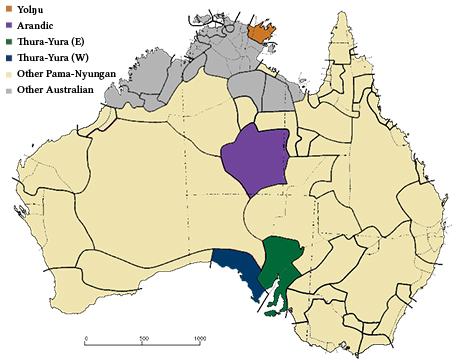
\includegraphics[scale=.7]{YolTYAr-leg.jpg}
	\caption[\textsc{map.} Pama-Nyungan subgroups investigated in Part \ref{NEC}]{Subgrouping of Australian languages. Pama-Nyungan family in tan, with Yolŋu subgroup given in ochre, Arandic in purple and Thura-Yura divided into green (Eastern varieties) and blue (Western/Nangga varieties.)}\label{Map}
\end{figure}

 Strategies that natural languages deploy to mark negation have long attracted the attention of philosophers and linguists \citep[see][]{Horn1989,Horn2010}. In a comprehensive piece of work on the subject, \citet[xiii--xiv]{Horn1989} observes that the ‘simplicity and transparency’ of logical negation (\textit{i.e.}, that function which ``reverses'' the truth value of a given proposition) is not recapitulated in ordinary language, where the complex behaviour of markers of negation and their interaction with other linguistic categories have long been investigated.\footnote{For \citet[1]{Horn2017}, \textit{negation} is basically the phenomenon of ``semantical opposition'' -- we are interested in that function which ``relates an expression $ e $ to another expression with a meaning that is in some way opposed to the meaning of $ e $.''}


 Recent work in the functionalist tradition (\citealp[\textit{e.g.},][]{Miestamo2005} a.o.) has sought to propose a typology for the behavior of `standard negation' marking strategies across a sample of world languages (including 40 Australian varieties.) \textit{\acrfull{sn}} is understood as those language-specific mechanisms whose function is the inversion of the truth value of a proposition associated with a given (declarative) clause. Drawing a distinction between \acrshort{sn} and `special negation' is warranted in view of the empirical fact that many languages have distinct formal mechanisms for the negation of nonverbal (\textit{e.g.}, copular, existential) predications, imperatives and other types of `subclausal' negation \citep{Miestamo2007,Horn2017,Veselinova2013,VanderAuwera2005}.
\subsection{Negation \& Australia: a typological snapshot}

Mentioned above, roughly 300 Australian languages have been reconstructed to a single family, Pama-Nyungan, spoken across Australia except for some regions in the north of the continent. The most recent common ancestor of these languages is esimated to have been spoken roughly five to six thousand years \textsc{BP} (a similar timedepth to Indo-European, see \citealt[742]{Bouckaert2018}). Many of these languages remain underdescribed, and consequently, typological and comparative work detailing the expression of negation across Australian languages is underdeveloped. Exceptions to this include \citealp{Dixon2002a} and \citealt{Phillips2021b}, surveys that have turned up some generalisations about the formal and functional expression of negation in these languages. Based on the insights of these works, we might divide the `negative semantic space' so to distinguish four macro-categories of negator: (1) negative imperatives/prohibitives, (2) clausal/standard negators and (3) nominal negators, including specialised negative existentials and a commonly occurring `privative' category, and (4) negative interjections. There is a substantial amount of variation in the formal exponence of each of these functions, some varieties distinguishing all four categories  (\textit{e.g.}, Bidjara [\gls{bym}]), some with a single syncretic marker for all four (e.g. Dyirbal [\gls{dbl}], according to \citealp[84--table 3.3]{Dixon2002a}). 

An exceptionful (but otherwise fairly robust) formal tendency across Australian languages is for clausal negation to be marked with a particle pre-verbally and for privative case to be encoded as a nominal suffix. We will explore the implications of this generalisation and its exceptions below, in a general overview of negation strategies in Australia, in addition to a deeper discussion of the meaning contribution of the so-called ``privative case'' markers in Australian languages. %The remainder of this section constitutes a brief survey the exponence of negation strategies in Australian languages, partially summarising insights from \citeauthor{PhillipsFCb} (forthcoming).
\subsection{``Standard'' negation}
This subection briefly provides some generalisations about clausal negation strategies in Australian languages. For a more comprehensive discussion of exceptions and significant interactions between \acrshort{sn} and other aspects of the verbal complex in Australian languages, the reader is referred to \citealt{Phillips2021b}.

\citet[82]{Dixon2002a} claims that ``almost every Australian language marks `not' by a non-inflecting particle which goes before the verb.'' He notes explicitly that this generalisation extends also to the most morphologically synthetic non-Pama-Nyungan languages spoken in the north of the continent. Negation in the Arandic subgroup of Pama-Nyungan, which provides a major exception (one of few) to this formal generalisation, and is particularly relevant for current purposes, is discussed in more detail in §\ref{ar}. The data from Nakkara ([\gls{nck}] Arnhem, Maningrida, \citealt[191]{Eather2011}) and Ngiyambaa ([\gls{wyb}] Pama-Nyungan: Wiradhuric) below clearly demonstrate this generalisation. In Nakkara \getref{sn-nck}, a preverbal negative marker \textit{korla} takes scope over a fully inflected verbal predicate (also affecting the inflectional suffix licensed by the verb, see also Ch. \ref{yolŋu} below.)
 In (\getfullref{sn-wyb.wyb1}), the preverbal SN particle \textit{waŋaːy} takes scope over the entire sentence (crucially including the discourse anaphor \textit{yingalaːdhi-} `because of that'), whereas it scopes underneath this item, over only the second predicate in (b), yielding two distinct propositions. 

\pex\begingl\glpreamble \textsb{Preverbal standard negation in Nakkara}\trailingcitation{\citep[191]{Eather2011}} \deftagex{sn-nck}//
\gla \textbf{Korla} nga-y-bburda-ma.//
\glb \textsc{\textbf{neg}} 1s.\gls{erg}-\gls{irr}-hit-\gls{infl}.\textsc{neg}//
\glft`I didn't hit him.'//\endgl\xe
\pex\deftagex{sn-wyb}\textsb{ Preverbal standard negation in Ngiyambaa}\trailingcitation{\citep[239]{Donaldson1980}}
\a\deftaglabel{wyb1}\begingl\gla \textbf{Waŋaːy} yiŋgalaː-dhi\textdblhyphen dju\textdblhyphen na girimiyi-la.//
\glb \textsc{\textbf{neg}} same-\textsc{circ}\textdblhyphen 1.\textsc{nom}\textdblhyphen3.\textsc{abs} wake\textsc{.pst-then}//
\glft`It wasn't because of that I woke her then.'//\endgl

\a\label{wyb2}\begingl\gla Yiŋgalaː-dhi\textdblhyphen dju\textdblhyphen na \textbf{waŋaːy} girimiyi-la.//
\glb same-\textsc{circ}\textdblhyphen 1.\gls{nom}\textdblhyphen3.\gls{abs} \textbf{\gls{neg}} wake.\gls{pst}-then//
\glft`Because of that I didn't wake her then.'//\endgl
\xe
\subsection{The ``privative case'' and existential predications}\label{priv-sems}

The privative case (\gls{priv}) is a very robustly attested category in Australian languages \citep[84]{Dixon2002a}.\footnote{Morphological cases with similar semantics are referred to as \textit{abessive} and/or \textit{caritive} in other literatures \citep[\textit{e.g.} for Uralic in][]{Hamari2011,Hamari2015,Tamm2015}. `Privative' is ubiquitous in Australian language description and will be used here throughout.} Broadly speaking, it predicates the absence of some property denoted by the noun that it associates with, although the precise semantic domain of this category varies considerably across languages \citep[\textit{cf.} arguments for the predicative status of negative existential markers in ][139]{Veselinova2013}. In Nyangumarta (\gls{nna} Pama-Nyungan: Marrngu), for example, \textit{-majirri} `\gls{priv}' can be used to predicate absence (\textit{i.e.} as a negative existential, see (\getref{nna-privEx}). Muruwari (\gls{zmu} Pama-Nyungan: SE) similarly makes use of a form \textit{-kil\textasciitilde-til\textasciitilde-tjil}, shown in (\getfullref{zmu-privEx}{a-b}).\footnote{Incidentally, \citet[77]{Oates1988} describes this suffix as the \textsc{abessive}: ``the opposite of the comitative in that it signifies `lacking' or `being without' some person of thing.' She glosses it throughout as `lacking.'}
\gls{priv} case markers are frequently antonymous to another case suffix, frequently occurring in Australian languages, usually glossed as the comitative (\gls{comit}), proprietive (\gls{prop}) or `\textit{having}' case. Uses of this marker are given in (\getref{ComEx}). The apparent synonymy of (\getref{zmu-privEx}b) and (\getref{ComEx}b) demonstrate the antonymous relation between comitative and privative predications.\footnote{The appendix to \citet{Singerman2018} comments on the instantiation of a very similar distribution in Tuparí ([\gls{tpr}] Tupian: NW Brazil), where the suffix \textit{-psiro} \textsc{`have'} is antonymous to \gls{priv} uses of the suffix \textit{-'om} `\gls{neg}'. }
%This function is clarified when contrasted against the `comitative/proprietive', another frequently occurring morpheme.


\pex\textsb{Function of \textit{-majirri} `\gls{priv}' in Nyangumarta}\deftagex{nna-privEx}\trailingcitation{\citep[140]{Sharp2004}}
\a\begingl\gla mungka-\textbf{majirri} karru-\textbf{majirri}-pa paru-\textbf{majirri} jungka jakun\deftaglabel{jungka}//
\glb tree\textbf{-\gls{priv}} stream\textbf{-\gls{priv}}-\gls{conj} spinifex\textsc{-\textbf{priv}} ground only//
\glft`There were no trees, creeks, or spinifex; only the ground (in that country.)'//\endgl
\a\begingl\gla mirtawa mayi-\textbf{majirri}\deftaglabel{mirtawa}//
\glb woman vegetable-\textbf{\gls{priv}}//
\glft`The woman is without food'//\endgl\xe
\pex~\textsb{Function of \textit{-kil} `\gls{priv}' in Muruwarii}\trailingcitation{\citep[77-8]{Oates1988} }
\a\begingl\gla palanj mathan\textbf{-kil}//
\glb nothing stick\textbf{-\gls{priv}}//
\glft`(There are no) sticks [...nothing]'//\endgl
\deftagex{zmu-privEx}
\a\begingl\gla ngapa\textbf{-kil}-pu-n//
\glb water-\textbf{\gls{priv}}-3\gls{s}-\gls{nmlzr}//
\glft`He has no water.' (lit. `he-waterless')// \endgl
 \xe
\pex~\textsb{Existential function of Muruwari \textit{-piɾa, -yita} `\gls{comit}'} \trailingcitation{\citep[73-4]{Oates1988}}
	\deftagex{ComEx}
\a\begingl%\glpreamble }//
	\gla thuu kuya-\textbf{yita} wartu//
	\glb much fish-\textsc{\textbf{comit}} hole.\gls{abs}//
	\glft`The river has a lot of fish in it.' (=There's a lot of fish in the river)//\endgl
	\a\begingl\gla wala mathan-\textbf{piɾa}//
	\glb \gls{neg} limb-\textbf{\gls{comit}}//
	\glft`(There are) no sticks.'//\endgl
\xe




Australian languages have a number of strategies to express existential and non-exis\-tence (absence) predications. (\getfullref{nna-privEx}) shows the Nyangumarta privative marker functioning as an existential negator: it predicates the absence of trees, streams and spinifex (a culturally important tussock grass) of a particular location. Additionally, \textit{contra} a prediction made by \citet[19]{Croft1991}, it is the case in many Australian languages that ``an existential sentence [can] consist solely of the noun phrase whose existence is predicated.'' Additionally, (\getfullref{nna-privEx}) includes an example of bare NP existential predication; the presence of \textit{jungka} `[bare] ground' (in the relevant location) is predicated.\footnote{Such constructions have also been reported elsewhere in the literature, \textit{e.g.}, for Māori [\gls{mao}] where ```existence'' statements have no copula or existence verbs' (\citealp[78]{Bauer1993}, cited by \citealp{Chung2004} a.o). Similarly, sign languages tend to allow bare-NP existential predication (see \citealt[26ff]{deWeert2016} on Flemish and Finnish sign languages.). Even Marra [\gls{mec}] (a language cited in \citealt[14]{Croft1991}) appears to permit bare NP existentials, if Heath's \citeyearpar[364]{Heath1981} translations are to be trusted.}
 These facts immediately present a challenge to the (formal) negative existential cycle as formulated: if existence predicates are frequently verbless, there is no way to formally distinguish between NEC stages $ \boldsymbol{\mathbb{A}} $ and $ \boldsymbol{\mathbb{C}} $ on the basis of synchronic data. I know of no Australian language with a \textit{reserved} existential verb; like copular clauses, existence predications appear to frequently make use of a stance or motion verb (most frequently one that primarily means `sit' or `lie' and often polysemous with `stay, live'), or are otherwise verbless.\footnote{Notable, however, is the fact that these stance/motion verbs often lend particular semantic nuances to the copular and existential predications in which they participate \citep[see e.g. ][610-611]{Wilkinson1991}.}

Relevantly for current purposes, then, the semantics of the privative suffix in this nonexistential use can be instructively captured by adapting existing analyses of existential propositions \citep[\textit{e.g.},][]{Francez2007,McNally2016}. These analyses generally characterise existential predication as comprising \textbf{obligatorily} some (type of) entity whose existence is being predicated (known as the \textsc{pivot)} and some \textbf{optional} restriction (perhaps locative) on its existence \citep[the \textsc{coda}; see][]{Francez2007}. Adapting Francez's analysis would mean treating privative noun phrases as generalised quantifiers of nonexistence. This is consonant with Croft's \citeyearpar[18]{Croft1991} observation about the privileged status of existential predication: representable as a logical quantifier as opposed to the one-place predicates of other stative verbs. For Croft, the relevant semantic distinction is that, where statives predicate a \textit{property} of a given individual, existentials are taken to ``[indicate] the presence or absence of the object itself.''  This observation --- an apparent conceptual distinction between the negation of a property versus the negation of existence --- forms the basis of functionalist explanation of the ``constant renewal'' of negative existentials at stage $\mathbb{B}$ of the NEC (see also \citealt[173]{Veselinova2016}).


In (\getref{Qdet}), I adapt Francez's quantificational treatment of existential predication in order to give a semantics for \textsc{priv} \citep{Francez2007,McNally2011}. Effectively, privative forms are taken to instantiate a negative quantificational determiner; they assert that the intersection of the two sets of individuals $ (P,\,Q\in\mathfrak D_{\langle e,t\rangle} )$ represented by their arguments is empty (\citealp[169]{Barwise1981}).

\pex \textbf{\gls{priv} realises a negative quantifier}
\deftagex{Qdet}\a$\textbf{no}=\lambda P_{\langle e,t\rangle}\lambda Q_{\langle e,t\rangle}.P\cap Q=\varnothing$%\hfill{\citep[i.e.,][169]{Barwise1981}}
\a $\llbracket\textsc{priv}\rrbracket=\lambda P_{\langle e,t\rangle}\lambda Q_{\langle e,t\rangle}.\textbf{no}(P,Q)$\xe


$ P $ and $ Q $ respectively represent those properties that can serve as the ``pivot'' and ``coda'' of an existential predication. Crucially $ Q $ need not have any syntactic representation, but is rather derived from context indexically (see \getfullref{nna-privEx.jungka}). This process, --- Francez's ``contextual closure'' \citeyearpar[72]{Francez2007}) --- is spelled out in (\getref{mungka}) below. Effectively, the variable $ Q $ over sets of individuals is saturated by a contextually given relation and discourse entity/set of parameters (\getref{francez-cc}).

\pex \textbf{Contextual domains of entities} \citep[from][71]{Francez2007}\deftagex{francez-cc}

For any element $ \alpha\in\mathfrak D_\tau$, $ \alpha $'s contextual domain is given as:
$$ d_\alpha\underset{\text{def}}{=} \lambda y_{\tau'}[\mathcal R_{\langle\tau,\langle\tau',t\rangle\rangle}(\alpha,y)]$$
That is, the set of individuals $ y\in\mathfrak D_{\tau'} $ that are related to $ \alpha_\tau $ by some pragmatically-inferred relation $ \mathcal R\subseteq \mathfrak{D_\tau\times\wp{(D_{\tau'})}} $

\xe

\noindent $ \mathcal R $ might be associated, for example with some relation \textbf{loc} which takes a set of salient spatiotemporal parameters (Francez suggests that this might be represented as a tuple $ st=\langle t,\ell\rangle $ and maps these to some set of entites \textbf{loc}ated within $ st $ (at that place, at that time.))

For Francez, the \textsc{coda}, then, plays the role of a ``contextual modifier'', the same type as a frame adverbial. In effect, it serves to explicitly provide that entity whose contextual domain satisfies $ Q $ (78). For example, in (\getfullref{nna-privEx.mirtawa}), the privative phrase is contextually ``closed'' by $ d_{\textit{mirtawa}} $ --- some set of things related (perhaps possessed) by \textit{mirtawa} `the woman.'


A truth-conditional analysis of one privative-marked noun (\textit{mungka} `tree') from (\getfullref{nna-privEx.jungka}) is provided in (\getref{mungka}) below; each step is spelled out in prose.

\pex \textbf{`There were no trees (in that country)': deriving (\getfullref{nna-privEx.jungka})}
\a\begingl\gla mungka-majirri//
\glb tree-\textsc{priv}//
\endgl
\a $\denote{\textit{mungka}}_{\langle e,t\rangle} =\lambda x_e.\textsf{Tree}(x) $
\a $\denote{\textit{mungka-majirri}}_{\langle\langle e,t\rangle,t\rangle}=\lambda Q_{\langle e,t\rangle}\big[\textbf{no}(\lambda x[\mathsf{Tree}(x)],Q)\big]$\label{privsemsF}\\
The privative-marked NP \textit{mungka-majirri} `tree-\gls{priv}' is a generalised quantifier: it states that there exists nothing in the domain in the intersection of the set of trees $(\lambda x.\textsf{Tree}(x))$ and some other property $ Q $ (which will be provided by the context of utterance, \textit{sc.} Francez's \textit{contextual domain} $d_\alpha$ \citeyearpar[71]{Francez2007}).
\a\textsb{Contextual closure}\par\nobreak

$\begin{aligned}\denote[c]{\textit{mungka-majirri}}&=\textbf{no}\big(\lambda x[\textsf{Tree}(x)],d_\alpha\big)\\
%&=\textbf{no}(\lambda x[\textbf{Tree}(x)],\lambda y[\textbf{loc}(st_c,y)])\\
&=\textbf{no}\big(\lambda x[\textsf{Tree}(x)],\lambda y[\textbf{loc}(st_c,y)]\big)\\\end{aligned}$\\
$ \boldsymbol Q $ is then saturated by $ d_{st_c} $: the ``set of things related [...] to the spatiotemporal parameters'' being predicated of (\textit{viz.} those things related to a particular patch of \textit{warrarn} `country' in the past, per Sharp's translation in (\getfullref{nna-privEx.jungka}))\hfill $ d_{st_{c}}=\lambda y_e.\mathcal R(\textsf{`that country'},y)$\deftagex{mungka}\deftaglabel{closure}

\xe

As (\getfullref{mungka.closure}) makes clear, in the absence of an explicit/linguistically-encoded ``coda'' to serve as a locus/restrictor for the privative predication, the \textbf{context} of utterance has made available an additional restriction ($ d_\alpha $) as the second argument to \textbf{no}. This restriction may take the form of a function \textbf{loc}, which returns that set of things which are taken to be related to whichever salient spatiotemporal parameters the context provides.


\subsection{Privatives and the \acrshort{NEC}}

If we treat the privative marking on NPs as a type of negative existential predicate, a consequence of the \acrshort{NEC} is the prediction that these markers ought to eventually generalise, displacing an erstwhile standard negator (\textit{i.e.}, \gls{priv}  markers will participate in the \acrshort{NEC}.) Phonological identity between privatives and SN is indeed well-attested in Australia (\textit{e.g.}, Bardi [\gls{bcj}] \citep{Bowern2012} and Warrongo [\gls{wrg}] \citep{Tsunoda2011}). In these languages, negative existential/privative predication may be syntactically distinguished from standard clausal negation by placing the general \gls{neg} particle post-nominally instead of preverbally (shown in (\ref{wrg-exx}) as well as (\ref{wgu-exx}a--b) below.)

\pex \textbf{Negation in Warrongo} (\texttt{[wgu]} Pama-Nyungan: Maric)\label{wrg-exx}
\a\begingl\glpreamble Senential negation with initial \textit{nyawa} `\textsc{neg}'//
\gla \textbf{nyawa} ngaya balga-lgo banjo-lgo.//
\glb \textsc{\textbf{neg}} 1\gls{s}.\gls{erg} hit-\gls{purp} ask\textsc{-purp}//
\glft`I will not hit [him]. [I] will ask [him].'\trailingcitation{\citep[363]{Tsunoda2011}}//\endgl

\a\begingl\glpreamble Existential negation with postnominal \textit{nyawa} `\gls{neg}'//
\gla nyawa, yarro walwa yamba. + yori \textbf{nyawa}, gajarra \textit{\textbf{nyawa}} worriba \textbf{nyawa}, barrbira \textbf{\textit{nyawa}}, jagay \textbf{\textit{nyawa}}.//
\glb \textsc{neg} this bad country. kangaroo \textsc{\textbf{neg}}, possum \textbf{\gls{neg}} sugarbag.bee \textbf{\gls{neg}} echinda \textbf{\gls{neg}} sand.goanna \textbf{\gls{neg}}//
\glft`No, this country is no good. There are no kangaroos, no possums, no bees, no echidnas, no sand goannas [in my country].'\trailingcitation{\citep[661]{Tsunoda2011}}//\endgl
\xe

 A possible example of a postnominal existential negator acquiring the function of clause-initial standard negator is found in Wirangu (\texttt{[wgu]} Pama-Nyungan: Thura-Yura). This scenario is described in \S~\ref{TY} below, along with a discussion of its potential import for theories of the \acrshort{NEC}.

\section{Negative domains \& the \acrshort{NEC} in three Pama-Nyungan subgroups}\label{empirical}

In this section, comparative and langauge-internal data from three subgroups of Pama-Nyungan, as they relate to the \acrlong{NEC}, are investigated.

§~\ref{TY} comprises a discussion of Thura-Yura --- a family spoken along the South Australian coast. In Thura-Yura, we observe a likely trajectory where a suffixal privative form appears to have developed into a preverbal standard negator \textit{maga}. In Wirangu, this has change created the conditions for the recruitment-by-borrowing of lexical material from an unrelated neighbouring language as a new privative.

§~\ref{NEC-yolŋu} consideres data from Yolŋu Matha, a family spoken in Eastern Arnhem Land. This section considers the competition and structured variation between two markers, \textit{yaka} and \textit{bäyŋu} --- the latter previously having been restricted to `negative quantifier' functions. In addition to this, we consider comparative evidence which suggests that in Djambarrpuyŋu privative marker \textit{-miriw} has expanded out of its traditional domain, to the extent that it is now showing signs of also being in competition with the preverbal negative particles. Conversely, the Ritharrŋu data show how a distinct sentential negative suffix \textit{-ˀmayˀ} appears to have been borrowed from a neighbouring language; a finding not predicted by (unidirectional) accounts of the NƎC.

Finally, §~\ref{ar} examines \acrlong{sn} as realised by negative suffixation in Arrernte; a typologically unusual feature for Australian languages. It is shown that negated clauses in Arrernte are actually derived (de-verbal) nominal predicates. This fact of Arrernte appears to provide strong evidence in favour of a trajectory where the standard negation strategy in this language is an erstwhile privative (negative existential) marker \textit{-tye\textdblhyphen kenhe} that has completely displaced an older form (and then triggered the recruitment of a new special negator for negative existential predications \textit{-kwenye}).




\subsection{Thura-Yura: change \& renewal in the negative domain}\label{TY}

Thura-Yura is a Pama-Nyungan language family, with nine documented varieties historically centered on and around the South Australian coast. The Western varieties of these languages abut the Wati (Western Desert) family. Figure \ref{TY-tree} describes the familial relations of the described Thura-Yura languages whereas Table \ref{TYdata} compares their negative lexica (including a possible reconstruction.) Examples of Wirangu negative predications are given in (\ref{wgu-exx}) below.\footnote{Note that \citep[57]{Hercus1999} describes a number of other markers with negative import in her Thura-Yura grammar (including two other lesser-used privatives, which she regards as older. \textit{Cf.} Veselinova's \citeyearpar[173]{Veselinova2016} ``constant renewal of the negative existentials.''}



	\begin{figure}[h]\centering
		\caption[\textsc{phylogeny.} Subgrouping in Thura-Yura]{A selection of the internal structure of the Thura-Yura family (spoken in South Australia) following \citealt[183]{Simpson2004}. \textit{Nangga} is the name given to the Western subgroup whereas core-ThuraYura refers to the Eastern varieties (see Figure \ref{Map} above for the approximate geographic distribution.)}\label{TY-tree}\small
	\begin{tikzpicture}
	\tikzset{edge from parent/.style=
{draw,
edge from parent path={(\tikzparentnode.south)
-- +(0,-8pt)
-| (\tikzchildnode)}}}
\tikzset{frontier/.style={distance from root=130pt}}

	 \Tree [.\textbf{\textit{\textsc{Thura-Yura}}} [.\textit{{\color{Blue}\textbf{Nangga}}} Wirangu Nauo ] [.\textit{{\color{OliveGreen}\textbf{core~TY}}} Nukunu  [.\textit{Yura} [Adnyamathanha Kuyani ] Bangarla ] [.\textit{Kadli} ] ] ] 
	\end{tikzpicture}\end{figure}
%\renewcommand{\arraystretch}{1}


Table \ref{TYdata} shows (colour-coded for cognacy) four of the negative-associated lexical items in the Thura-Yura family, each of which will be discussed here. It allows for a probable reconstruction of a standard negator (or nominal negator) \textit{*maka} and/or \acrshort{sn} \textit{*guda} in the ancestral language. Of Wirangu \texttt{[wgu]}, \citet[57]{Hercus1999} claims that privative morpheme \textit{-yudu} has entered the language as a borrowing from the Kokata language, a Western Desert dialect spoken in neighbouring territories to the North ([\gls{ktd}] Pama-Nyungan: Wati). \textit{-yudu} has largely displaced \textit{-maga} as the form of the privative. The recruitment of a distinctive privative form (from lexical resources of a neighbouring, unrelated language) may well be taken as evidence of pressure for the privileged marking of negative existentials that is taken to motivate the beginning of the NEC (\textit{sc.} stage transition $A\to B$).

\begin{table}[H]\centering
	\caption[Lexicalisation of the negative domain in Thura-Yura]{Reported partitions in the negative semantic space (data adapted from \citealt{Hercus1999,Hercus1992,Schurmann1844,Hercus1996,Black1917}.) Colouring reflects hypothesised cognacy of lexical items across Thura-Yura. Dashed arrows represent borrowings from neighbouring languages, solid arrows semantic (functional) change.} \label{TYdata}
\begin{tabular}{r|c|c|c}\toprule
\textit{\textsc{\scriptsize(Wa}}\tikzmark{o}{\centering\scriptsize\textit{\textsc{t}}}\textit{\textsc{\scriptsize i)}}	& \gls{negq}/\gls{priv} & \acrshort{sn} & {\small`cannot'/`not yet'} \\ \toprule
Wirangu [\gls{wgu}] & \begin{tabular}[c]{@{}l@{}}\tikzmark{c}{\textit{\textcolor{teal}{-yudu}}}\\ \textcolor{violet}{\textit{-maga}}\tikzmark{d}\end{tabular}   & \tikzmark{b}\textcolor{violet}{\textit{maga}}   & \textcolor{brown}{\textit{guda}}   \\ \midrule
Nauo [\gls{nwo}] & ? & \textcolor{violet}{\textit{makka}} & \\\midrule
Bangarla [\gls{bjb}] & \textcolor{violet}{\textit{-maga}}  & \textcolor{violet}{\textit{makka}}  & \tikzmark{a} \textcolor{brown}{\textit{kutta}}\\ \midrule
\begin{tabular}[c]{@{}r@{}}Adnyamathanha [\gls{adt}]\\Kuyani  [\gls{gvy}]\end{tabular} & \tikzmark{pari}{\textit{pari- }}  & \textcolor{brown}{\textit{(g)uda}}   & \tikzmark{e}--\tikzmark{ee}   \\\midrule
Nukunu [\gls{nnv}] & \textcolor{violet}{\textit{-wakanha}$ ^? $} & & \\\midrule
\textit{proto-TY} & \multicolumn{3}{c}{\textit{\textcolor{violet}{\textbf{*maka}}/\textcolor{brown}{\textbf{*guda}}}} \\\bottomrule
{\scriptsize{\textcolor{gray}{\textit{\textsc{Diyari?}} ([\gls{dif}] Karnic)}}}\tikzmark{dif}
\end{tabular}

\begin{tikzpicture}[overlay,remember picture, shorten >=1pt]
\draw[->,yshift=3ex,xshift=1ex, color=teal,dashed] (pic cs:o) to[bend right] (pic cs:c) ;
\draw[->,xshift=-3ex,yshift=.5ex, color=violet] (pic cs:d) -- (pic cs:b);
%\draw[->,xshift=0.7ex] (pic cs:ee) -- (pic cs:b);
\draw[->,color=gray,dashed,out=0,in=180] (pic cs:dif) to[] (pic cs:pari);
\end{tikzpicture}\end{table}

%%%% THIS IS THE ORIGINAL SUBFIGURE FORMAT THAT REVIEWER X HAS SOME PROBLEM WITH.
%\begin{figure}[h]
%	\caption{Change in the negation domain across Thura-Yura languages}\label{TY-data}
%	\begin{subfigure}{.4\textwidth}
%		\caption{A selection of the internal structure of the Thura-Yura family (spoken in South Australia) following \citealt[183]{Simpson2004}}.\small
%		\Tree [.\textbf{\textit{Thura-Yura}} [.\textit{Nangga} \gls{wgu} \gls{nwo} ] [.\textit{core~TY} [.\gls{nnv} ] [.\textit{Yura} [\gls{adt} \gls{gvy} ] \gls{bjb} ] [.\textit{Kadli} ] ] ] 
%	\end{subfigure}
%	%\renewcommand{\arraystretch}{1}
%	\begin{subfigure}{.5\textwidth}
%		\caption{Reported partitions in the negative semantic space (data adapted from \citealt{Hercus1999,Hercus1992,Schurmann1844,Hercus1996,Black1817}.) Colouring to reflect hypothesised cognacy of lexical items across Thura-Yura.} \label{TYdata}
%		\begin{tabular}{r|c|c|c}\toprule
%			\tikzmark{o}	& \textsc{negq/priv} & SN & {\small`cannot'/`not yet'} \\ \toprule
%			Wirangu [\gls{wgu}] & \tikzmark{c}\begin{tabular}[c]{@{}l@{}}\textit{\textcolor{teal}{-yudu}}\\ \textcolor{violet}{\textit{-maga}}\tikzmark{d}\end{tabular}   & \tikzmark{b}\textcolor{violet}{\textit{-maga}}   & \textcolor{brown}{\textit{guda}}   \\ \midrule
%			Nauo [\gls{nwo}] & ? & \textcolor{violet}{\textit{makka}} & \\\midrule
%			Bangarla [\gls{bjb}] & \textcolor{violet}{\textit{-maga}}  & \textcolor{violet}{\textit{makka}}  & \tikzmark{a} \textcolor{brown}{\textit{kutta}}\\ \midrule
%			\begin{tabular}[c]{@{}r@{}}Adnyamathanha [\gls{adt}]\\Kuyani  [\gls{gvy}]\end{tabular} & \textit{pari- }  & \textcolor{brown}{\textit{(g)uda}}   & \tikzmark{e}--\tikzmark{ee}   \\\midrule
%			Nukunu [\gls{nnv}] & \textcolor{violet}{\textit{-wakanha}} & & \\\midrule
%			\textit{proto-TY} & \multicolumn{3}{c}{\textit{\textcolor{violet}{\textbf{*maka}}/\textcolor{brown}{\textbf{*guda}}}} \\\bottomrule
%		\end{tabular}
%		
%		\begin{tikzpicture}[overlay,remember picture, shorten >=1pt]
%		\draw[->,yshift=2ex,xshift=-1.5ex] (pic cs:o) -- (pic cs:c) ;
%		\draw[->,xshift=0ex,yshift=.5ex] (pic cs:d) -- (pic cs:b);
%		%\draw[->,xshift=0.7ex] (pic cs:ee) -- (pic cs:b);
%		\end{tikzpicture}\end{subfigure}\end{figure}





\pex \textbf{Examples of Wirangu negation strategies (from \citealt{Hercus1999})}\label{wgu-exx}
\a\begingl\glpreamble \textsb{\em{maga} SN}//
\gla Warlba marnaardu-nga \textbf{maga} wina-rn!//
\glb wind big\textsc{-loc} \textsc{\textbf{neg}} go\textsc{-pres}//
\glft `(I am) not going out in a gale!'\trailingcitation{(142)}//\endgl

\a\begingl\glpreamble \textsb{\em{-maga} privative}//
\gla Nganha gidya\textbf{-maga}//
\glb 1\gls{s} child-\textsc{\textbf{priv}}//
\glft`I haven't got any children.'\trailingcitation{(57)}//\endgl

\a\begingl
\glpreamble\textsb{ \em{-yudu} privative }(``most commonly used'')//
\gla Nganha barnda-\textbf{yudu}//
\glb 1\gls{s} money-\textsc{\textbf{priv}}//
\glft`I haven't got any money.'\trailingcitation{(57)}//\endgl

\a\begingl\glpreamble \textsb{\em{guda} SN (modalised)}//
\gla Ngadhu \textbf{guda} wangga-rn//
\glb 1\gls{s}.\textsc{erg} \textsc{\textbf{neg.}irr} speak\textsc{-pres}//
\glft`I can't talk (about this; it's too embarassing.)'\trailingcitation{(143)}//\endgl
\xe


 Similarly, Adnyamathanha [\gls{adt}] and Kuyani [\gls{gvy}] have recruited \textit{pari-} as a negative existential/predicator of absence \citep[141]{Hercus1999}. This may also be a borrowing from the Karnic lanugages that abut Eastern Thura-Yura (e.g. Diyari [\gls{dif}] \textit{pani} \textsc{`priv'}, (\citealt{Austin2011}, {C. Bowern \textit{p.c.}).\footnote{This remains to be demonstrated, but \textit{pari-} may otherwise be cognate with Wirangu \textit{bal-} `die,' elsewhere described as a lexical source for negators (\citealt{Veselinova2013}, van Gelderen this volume). An argument potentially in favour of this is found in a possibility of an example of lexical renewal likely born of euphemism; Adnyamanthana \textit{inta-} `die' appears to be cognate with Wirangu \textit{inda-} `spill.'}
\textit{maga} retains its function as the primary standard negator particle in Wirangu (and Bangarla [\gls{bjb}]),  whereas \textit{guda} (the standard negator in Adnyamathanha and Kuyani), is restricted to a subset of negative meanings: `cannot' and `not yet' (note that, particularly in northern Australia, the form of negative marking is often conditioned by speaker mood/reality status (see Part \ref{yolngu}, esp. \S~\ref{sec:yol-mood} for an example of a related phenomenon.)

A potential cognate in the southern Thura-Yura (Kadli) language, Kaurna [\gls{zku}] (not represented in Figure \ref{TY} for a lack of available data) \textit{wakka-} is found (possibly fossilised) in lexical items \textit{wakkarendi} `err, stray, be lost', \textit{wakkariapendi}, `forget, not think of, leave behind', \textit{wakkariburka} `ignorant person, simpleton' \citep[II-52]{Schurmann1840}.\footnote{Note attested stems in \textit{pia\textbf{-rendi}} `scattered, stray', \textit{pia\textbf{-riappendi}} `scatter, disperse', \textit{\textbf{burka}} `adult, man' \citep[II-4,38]{Schurmann1840}.} All three of these words appear to be analysable; \textit{wakka-} contributing some notion of emptiness, characteristic of an erstwhile nominal negator/privative category. Apparently, \citeauthor{Teichelmann1840} (1840, cited in \citealt{Amery1996a}) give \textit{mukandariappendi} as the form for `forget' --- support for potential \textit{m\textasciitilde{w}} alternation and the cognacy of these forms.\footnote{Data for Kaurna (and other extinct varieties) is scarce, effectively limited to the lexica published by nineteenth-century missionaries, \citet{Schurmann1840}. A possible reflex of \textit{*guda} is found in items like \textit{kudmunna} `ignorant, not knowing' (II-12). Additionally, Narungga \textit{-gu} (potentially a ``compound form'') appears in a number of words with a meaning akin to `blocked', according to \citet[82]{Eira2010}. Notably, compare \textit{mina-gu} `blind' (lit. `eye-blocked') where the semantic connection to an inability/impossibility reading is clear.
	
	Other negative lexical items reported here are \textit{yakko} which appears to function as a SN marker and \textit{-tinna} which is given as the most frequent form of `without' (i.e. the privative.)}

 There are insufficient available data to adjudicate between competing hypotheses that (a) \textit{*guda} has been largely displaced by erstwhile nominal negator \textit{maga} in Wirangu or (b) \textit{guda} has replaced \textit{*maka} in Adnyamathana/Kuyani. Nevertheless, an analysis informed by the insights of the \acrshort{NEC} favours and supports (a).
 
Under such an analysis, Wirangu -- the Thura-Yura outlier -- provides a particularly clear example of a language, the negator forms of which are transitioning through the NEC. The erstwhile negative existential \textit{-maga} has entered the domain of standard, clausal negation, adopting the morphosyntactic properties of a preverbal negative (stage $\mathbb{B\to C}$),\footnote{Note that, while this change is consonant with functional grammaticalisation ``generalisation'', the transition from bound- to free-form is perhaps surprising in view of the (controversial) claim that grammaticalisation clines involve processes of phonetic reduction and syntactic ``rigidification'' (e.g. \citealp{Geurts2000}). If the account described here is on the right track, the trajectory of \textit{maga} in Wirangu constitutes a counterexample of these grammaticalization ``form'' paths (see \citealp[40]{vanderAuwera2008,Ahern} for the dissociation of ``formal'' and ``functional/semantic'' grammaticalisation processes).} and triggering the recruitment of a new privative marker from the lexical resources of a neighbouring language \textit{-yudu} which is now in competition with the old marker (stage $\mathbb{A\to B}$). The ostensible simultaneity of these changes also provides further evidence for competition between functional and formal pressures for generalisation and recruitment (\textit{sc.} Veselinova's ``constant renewal of the negative existential'' \citeyearpar[173]{Veselinova2016}).
\citealt[225]{Miestamo2005}, \citealt{Phillips2021b}.)%todo\marginnote{there's sth strange going on w the T\&S sourcing here, i'm not totally sure who says what \& may need to go back to archives to find out.}

Additionally, if the directionality of change described here is indeed on the right track, Wirangu can be shown to resist classification into any unique \acrshort{NEC} `stage', transitional or ``cardinal'' (in which case the NEC as described in previous work does not represent a complete linguistic typology for negative existential marking strategies.)\footnote{The issues of ``assigning'' the entire negative domain of a given language to a unique stage in the \acrshort{NEC} have been explored in some detail by \citep{Veselinova2016}, who observes similar classificatory issues for a number of languages (\textit{e.g.}, East Futunan [\texttt{fud}]: Polynesian).}










\subsection{The Yolŋu negative domain}\label{NEC-yolŋu}

The Yolŋu languages, a Pama-Nyungan grouping of at least six dialect clusters (roughly coterminous with sociocultural groupings) are spoken through Eastern Arnhem Land (in the far north of the continent) by some 12,000 Aboriginal inhabitants (see Part \ref{yolŋu} of the current dissertation, also \citealt[18\textit{ff}]{Wilkinson1991}). Yolŋu are strictly exogamous -- each cultural group (clan) being associated with a distinct dialect, a situation that has led to a significant amount of stable linguistic variation (and, consequently, undetermined internal classification; see \S~\ref{sec:yol-bkgrd}, also  \citealt{Schebeck2001}, \citealt[836]{Bowern2012b}).
%todo intro ch for more ym

This section compares the negation systems of three distinct Yolŋu varieties: Djambarrpuyŋu [\gls{djr}], Ritharrŋu [\gls{rit}] and Wangurri [\gls{dhg}] in view of making inferences about change in marking strategies over time. A pattern similar to that observed in Thura-Yura is shown. The key findings are tabulated in Table \ref{compYol} below. The final subsection (§\ref{yolpriv}) comprises a discussion of privative case semantics with particular reference to Yolŋu.

\begin{table}[h]
	\centering
	\caption[Lexicalisation of the negative domain in three Yolŋu Matha varieties]{Partitioning of the negative space in three Yolŋu languages.\\`\gls{proh}' negates imperatives, \gls{sn} represents `standard negation'. `\gls{priv}' is taken to denote a suffix of the type described above. `\gls{negq}' (Wilkinson's ``negative quantifier'') are independent words that appear to quantify over the NP which they modify (\textit{i.e.}, perform (minimally) the same work as a \gls{priv} suffix.)}
	\label{compYol}
	\begin{tabular}{lrllll}
		&& {\sc proh}                                                     & {\sc sn}                                                         & {\sc negq}                                             & {\sc priv} \\\toprule\toprule
		\textbf{Djambarrpuyŋu} & \gls{djr} & \textit{yaka}                                                             & \begin{tabular}[c]{@{}l@{}}\textit{yaka}\\ \textit{bäyŋu}\end{tabular}               & \textit{bäyŋu}                                                     & \textit{-miriw}       \\\midrule
		\textbf{Ritharrŋu} &\gls{rit} & \textit{yaka}                                                             & -\textit{ˀmayˀ}                                                             & \textit{yakaŋu}                                                    & \textit{-miriw}       \\\midrule
		\textbf{Wangurri} &\gls{dhg} & \begin{tabular}[c]{@{}l@{}}\textit{yaka}\\ \textit{ŋangawul}\\ \textit{bayaŋu}\end{tabular} & \begin{tabular}[c]{@{}l@{}}?\textit{yaka}\\\textit{ŋangawul}\\ ?\textit{bayaŋu}\end{tabular} & \begin{tabular}[c]{@{}l@{}}\textit{ŋangawul}\\ \textit{\textit{bayaŋu}}\end{tabular} & \textit{-nharra}  \\\bottomrule   
	\end{tabular}
\end{table}


\subsubsection{Djambarrpuyŋu}\label{sec:nec-djr} \textbf{Djambarrpuyŋu} [\gls{djr}] appears to provide an example of Croft's $B\sim C$ transitional-stage language. \citet[356]{Wilkinson1991} describes the coexistence of two markers: \textit{yaka} `\gls{neg}' and \textit{bäyŋu} `\gls{negq}' (negative quantifier): claiming that `both occur as propositional negators,' demonstrated in the data in (\nextx) below, from \citet{Wilkinson1991}.

\pex\textbf{\acrlong{sn} in Djambarrpuyŋu}
\a\begingl\glpreamble \textit{{\em yaka} as (full) clausal negator}//
\gla \textbf{yaka} ŋayi dhu ga ŋutha-n ŋaṉḏi-wal bäpa-wal//
\glb \textsc{\textbf{neg}} 3\gls{s} \textsc{fut} \gls{ipfv}.\gls{I} grow-\textsc{I} mother\textsc{-obl} father\textsc{-obl}//
\glft `They don't grow up with (their) mother and father.'\trailingcitation{\citep[691]{Wilkinson1991}}//
\endgl
\a\begingl\glpreamble \textit{{\em yaka} as negator in attributive (nonverbal) predication}//
\gla \textbf{yaka} dhuwali ŋatha, dhuwali ŋula nhä-n dhuwali botjin//
\glb \textsc{\textbf{neg}} \gls{med} food \gls{med} \textsc{indef} what-\textsc{seq} that poison//
\glft`That isn't food, that's something else, that's poisonous.'\trailingcitation{\citep[560]{Wilkinson1991}}//\endgl
\a\begingl\glpreamble yaka \textit{as negator in possessive construction}//
\gla warrakan limurruŋ \textbf{yaka} dhuwal//
\glb animal 1\gls{p}.\textsc{incl.dat} \textbf{\gls{neg}} \gls{prox}//
\glft`This meat isn't ours/for us.'\trailingcitation{[AW~20190505]}//\deftagex{yaka}\deftaglabel{meat}
\endgl
\a\begingl
\glpreamble\textit{ {\em bäyŋu} as clausal negator}//
\gla \textbf{bäyŋu} ŋarra gäthur ŋorranha manymak-kunha munhawu//
\glb \textsc{\textbf{negq}} 1\gls{s} today lie.\gls{IV} good-\gls{tr}.\gls{IV} night//
\glft `I didn't sleep well last night.'\hfill\citep[357]{Wilkinson1991}//
\endgl\deftagex{djr-yaka}\xe

The distributional difference between these two markers is twofold. According to Wilkinson, \textit{yaka} is ungrammatical in quantificational contexts and that \textit{bäyŋu} does not appear in imperative (\textit{i.e.} prohibitive) contexts. It seems, then, likely, that in Djambarrpuyŋu, \textit{bäyŋu}, an erstwhile negative existential has begun to encroach further into the negation space, entering into competition with \textit{yaka}. \textit{bäyŋu}, with reflexes in other Yolŋu languages, derives from (fairly productive) verbal root \textit{bäy-} `leave.'\footnote{Note also that \textit{-\textsc{th}i} `\gls{inch}' derives absence-associated change-of-state readings: \textit{bäy-thi} `be left over/behind'; \textit{bäyŋu-thi} `be/have none, pass~away, die' \citep[378]{Wilkinson1991}. The semantics of this suffix is investigated in \S~\ref{sec:djr-prs}.} Examples of negative existential uses of \textit{bäyŋu} are given in (\nextx) and prohibitive uses of \textit{yaka} in (\anextx).


\pex\deftagex{bayŋu-negq} \textbf{Djambarrpuyŋu negative quantification}
\a\begingl\gla dhipuŋur-nydja \textbf{bäyŋu} guku//
\glb \gls{med}.\gls{abl}-\gls{prom} \textbf{\gls{negq}} honey//
\glft`From this (tree) there's no honey.'\trailingcitation{\citep[554]{Wilkinson1991}}//\endgl

\a\begingl
	\gla (*yaka/)\textbf{bäyŋu} ŋarra-ku gi ŋorri ŋula dhiyal wäŋa-ŋur-nydja//
	\glb \textsc{*neg/\textbf{negq}} 1\gls{s}\textsc{-dat} \gls{ipfv}.\gls{II} lie:\gls{II} \gls{indef} \gls{prox}.\gls{loc} place-\textsc{loc-foc}//
	\glft`I don't have any here' (lit. `at this place lie (are) none of mine')\trailingcitation{\citep[691]{Wilkinson1991}}//
	\endgl
\a\begingl\gla bili ($^\#$yaka/)\textbf{bäyŋu} limurruŋ dhuwal bäwarraṉ//
\glb because \textsc{$^\#$neg/\textbf{negq}} 1\gls{d}.\textsc{incl.dat} \textsc{prox} animal//
\glft\textbf{Intended reading:} `Because there's no meat for us.'\trailingcitation{(\citealp[560]{Wilkinson1991}, infelicity judgment \textsc{aw20190505}, cf. \lastx c)}//\endgl\deftagex{djr-bayŋu}\deftaglabel{meat}
\xe

\noindent Note in particular the (obligatory) contrast in the interpretation of (\getfullref{djr-bayŋu.meat}) as against (\getfullref{yaka.meat}) where the semantics of \textit{bäyŋu} and \textit{yaka} come apart. Only the former is available as a negative quantifier (that is, on the negative existential reading.)


\pex\deftagex{yaka}\begingl\glpreamble\textbf{Djambarrpuyŋu imperative negation (prohibitive, see also §\ref{yolpriv})}//
\gla \textbf{yaka(/*bäyŋu)} waŋi!//
\glb \textsc{\textbf{neg}(/*negq)} talk.\gls{II}//
\glft`Don't talk!'\trailingcitation{\citep[360]{Wilkinson1991}}//\endgl\xe


There are multiple arguments for a reconstruction of \textit{*yaka} `\gls{neg}' to proto-Yolŋu. First is the fact that it is reported as a negative particle in all Yolŋu varieties \citep[31]{Schebeck2001}.

 Secondly, possible lexical cognates are reported in likely sisters to Yolŋu in the Western Pama-Nyungan subfamily (a monophyletic branch reconstructed in \citealt[838]{Bowern2012}). \citet[226]{Sharp2004} and \citet[67]{Ogrady1963} both report a Nyangumarta ([\gls{nna}] W. Pama-Nyungan: Marrngu) verb \textit{-yaka-} meaning `leave, quit.' \citet[35]{Mckelson1974} additionally gives \textit{yaga} as an alternative (potentially emphatic) negative particle in Mangala ([\gls{mem}] Marrngu). It is very possible that these Marrngu verbs are cognate with the Yolŋu negator, despite Marrngu and Yolŋu having been distantly separated for centuries. Further, \citet[85]{Dixon2002a} lists other potential cognates to negative \textit{yaka} from a number of other dispersed Pama-Nyungan languages.
 
 Thirdly, the generalisations of the NEC as formulated by \citet{Croft1991} and \citeauthor{Veselinova2016} (2016 a.o.) provide a principled typological basis through which an erstwhile negative existential construction arises in a language and begins to encroach upon the functional domain of a standard (clausal) negator (transitional stage $\mathbb{B\sim C}$.) If this diachronic analysis is on track it may have implications for our understanding of the characteristics of stage $\mathbb{B\sim C}$: negative imperatives (prohibitives) being one of the last `holdouts' for an erstwhile SN marker that is threatened by competition from a negative existential or quantifier. %\footnote{Although such an account would require further nuance given data like (\getfullref{miriw}i) \textit{infra}.}
 Dixon's typology \citeyearpar[84]{Dixon2002a} indeed entails an implicational relationship: if there is formal syncretism between privative and prohibitive marking, then these will be syncretic with the \gls{sn} marker as well. Gumbaynggir ([\gls{kgs}] Pama-Nyungan: Southeast; \citealt{Eades1979}) and Nyawaygi ([\gls{nyt}] Pama-Nyungan: Dyirbalic; \citealt{Dixon1983}) are given as examples of a languages for which the prohibitive patterns distinctly from all other negative functions (a datum which is a potential indicator of a language in NEC stage $\mathbb{B\sim C}$). The Ritharrŋu data presented in §\ref{secrit} below raise a potential counterexample.
\label{secdjr}

\subsubsection{Ritharrŋu}\label{secrit}


The facts outlined in Heath's description of {\bf Ritharrŋu} (\gls{rit}, \citeyear{Heath1980}) diverge in a number of significant ways from the Djambarrpuyŋu situation described above. Further, they appear to pose a potential problem for the generality/predictive power of the NEC as formulated.\footnote{Data provided from \citet{Heath1980} has been standardised to an Australianist (Yolŋu) orthography from his original IPA transcription.} While a form \textit{bayŋu} has been retained in the language (glossed as `nothing'), there is an additional suffixal form \textit{-ˀmayˀ} used as the ``basic'' \citep[101]{Heath1980} general negator alongside \textit{yaka} (the latter form is the standard means of forming prohibitives in Ritharrŋu, shown in \ref{ritproh}).

\pex\textbf{Standard and copular negative suffixation of {\em -ˀmayˀ} in Ritharrŋu}
\a\begingl\gla wäni-na\textbf{-ˀmayˀ} napu//
\glb go-\textsc{pst-\textbf{neg}} 1\gls{p}.\gls{excl}//
\glft `We didn't go.'//\endgl
\a\begingl\gla munaŋa-\textbf{ˀmayˀ} rra//
\glb white.fellow\textsc{\textbf{-neg}} 1s//
\glft`I'm not white'\trailingcitation{\citep[101]{Heath1980}}//\endgl\xe 
\pex~\label{ritproh}\begingl\glpreamble\textsb{Prohibitive formation with {\em yaka} in Ritharrŋu}//
\gla \textbf{yaka} nhe baŋgurlˀ-yu-ru//
\glb \textsc{\textbf{neg}} 2\gls{s} return-\textit{them}-\textsc{fut}//
\glft`Don't come back!'\trailingcitation{\citep[76]{Heath1980}}//\endgl\xe

Existential negation, however, is introduced by the complex form \textit{yaka-ŋu} (shown in \nextx{} below). This form is clearly related to the Djambarrpuyŋu SN particle described above, with archaic Yolŋu suffix {\textit{-ŋu}} (described as an `adjective $\Rightarrow$ substantive' derivation by \citet[34]{Schebeck2001}, see also \citealt[174ff]{Wilkinson1991}, \citealt[24]{Heath1980}.) Heath glosses \textit{yakaŋu} as a particle meaning `absent' \citeyearpar[102]{Heath1980}.\footnote{Note that Heath also points out that stance predicates with copular/existential readings can also receive negative marking as in (\nextx{b}$^\prime$) below. 
	\pex[exno=\ref{ritnegxb}′,numoffset=3em]~\begingl\gla nhiena-\textbf{ˀmayˀ} ŋay yaŋˀ-ŋarṛa//
	\glb sit\textsc{.pres\textbf{-neg}} 3\gls{s} here//
	\glft`He isn't (sitting) there'\trailingcitation{\citep[102]{Heath1980}}//\endgl \xe
}
Recalling the possible lexical sources of pan-Yolŋu form (Table \ref{compYol} \textit{supra}) \textit{*yaka} discussed in the foregoing section, this is an appropriate translation.

%It is notable additionally, however, that Heath points out that the neighbouring (but genetically unrelated) language, Ngandi, shares this form \citeyearpar[101]{Heath1980}. Heath asserts that \textit{-ˀmayˀ} has been borrowed into Ritharrnu from Ngandi, but in view of this discussion, this claim may be worthy of reassessment.} Such an analysis finds support in the fact that (1) \textit{-bay'} persists in the language as a question tag particle and additionally (2) \textit{-ŋu} is present across multiple Yolŋu languages and may be related to a formerly productive nominal/adjectival suffix.\footnote{This is like the same \textit{*-ŋu} that is no longer analysable in \textit{yolŋu} (p.c. Claire Bowern.)}
\pex\textbf{Existential negation with {\em yakaŋu} in Ritharrŋu}
\a\begingl\gla \textbf{yakaŋu} ŋay dhäŋgu//
\glb\textsc{\textbf{negq}} 3\gls{s} meat//
\glft`There's no meat.'\trailingcitation{\citep[102]{Heath1980}}//
\endgl
\a\label{ritnegxb}\begingl\gla \textbf{yakaŋu} ŋay (yaŋˀŋara)//
\glb \textsc{\textbf{negq}} 3\gls{s} (here)//
\glft`He isn't here'\trailingcitation{\citep[102]{Heath1980}}//\endgl
\xe

While it may be tempting to relate \textit{bäyŋu}, as found in other Yolŋu languages, to a possibly lenited form \textit{-ˀmayˀ}, as \citet[102]{Heath1980} points out, it is much more likely to be a borrowing from the geographically neighbouring language Ngandi [\gls{nid}], an unrelated, non-Pama-Nyungan language also spoken in southeastern Arnhem for which \textit{-ˀmay} is a fusional negative-cum-present tense suffix. The structure of the negative domain in Ritharrŋu (\textit{i.e.}, the use of \textit{‑ˀmayˀ} in (zero-)copular} clauses (\bblastx{a}) and the apparent unavailability of \textit{‑ˀmayˀ} in quantificational/existential predications) provides support for the borrowing account, which is considerably more parsimonious than an account by which the syntax, semantics, phonology and perhaps morphology  of \textit{bäyŋu} were radically reorganised into a SN suffix.
%\footnote{The structure of the Ritharrŋu negative domain (\textit{i.e.} the use of \textit{-ˀmayˀ} in (zero-)copular clauses and ostensible unavailability in quantificational/existential predications) provides support for the borrowing account, which is consequently considerably more parsimonious than an account by which the syntax, semantics, phonology, and perhaps morphology of \textit{bäy(ŋu)} were radically reorganised.}
If this is indeed the case, the trajectory runs counter to hypotheses of a unidirectional \acrshort{NEC} (\textit{e.g.}, \citealt[146]{Veselinova2016}): an innovative \textit{standard negator} has been recruited into Ritharrŋu's negative space, whereas the so-called ``special negators'' have retained an older form (Figure \ref{RitNEC}).


\begin{wrapfigure}{r}{.25\textwidth}
	\caption[Innovative standard negation in Ritharrŋu]{\footnotesize Not predicted by the \acrshort{NEC}, Ritharrŋu appears to have recruited an innovative clausal negator $\neg^\prime$  into negative space. This is likely to be an effect of extended contact with an unrelated non-PN language (Ngandi [\gls{nid}]).}\label{RitNEC}
	\footnotesize\centering\begin{tikzpicture}[scale=0.2]
	\tikzstyle{every node}+=[inner sep=0pt]
	\draw [black] (23.6,-7.9) circle (3);
	\draw (23.6,-7.9) node[rectangle split,rectangle split parts=2] {\textbf{A}\nodepart{second} $\neg\phi/\neg\exists x$};
	\draw [black] (23.6,-22.1) circle (3);
	\draw (23.6,-22.1) node[rectangle split,rectangle split parts=2] {\textbf{B$^\prime$}\nodepart{second} $\neg^\prime\phi/\nexists x$};
	\draw [-{Latex[length=2.8mm,width=2.5mm,black]},white, snake it] (23.6,-10.9) -- (23.6,-19.15);
	\draw [black, snake it] (23.6,-10.9) -- (23.6,-17.6);
	%\fill [black] (23.85,-19.1) -- (24.35,-18.3) -- (23.35,-18.3);
	\end{tikzpicture}	
\end{wrapfigure}



 Whatever the providence of \textit{-ˀmayˀ}, this is the marker of standard clausal negation whereas existential negation appears to be obligatorily marked by \textit{yakaŋu.} Incidentally, on the basis of the limited data presented here, Ritharrŋgu, a language closely related to Djambarrpuyŋu, might \textit{synchronically} be described as a stage $\mathbb B$ language \textit{per} the negative existential typology described in this volume, although such a description plasters over the likely diachronic trajectory of Ritharrŋu negative marking.



\subsubsection{Wangurri}

Finally, negation in \textbf{Wangurri} {\tt[dhg]}, a northern Yolŋu dialect, appears to make use an additional particle with the semantics of a general negator, \textit{ŋangawul} in addition to \textit{yaka} and \textit{bayaŋu}. \citet[195]{McLellan1992} claims that \textit{ŋangawul} and \textit{bayaŋu} can be used in all negative contexts and that \textit{yaka} cannot be used as a ``negative quantifier.'' These data are exemplified in (\nextx) below, all adapted from \citet{McLellan1992}.

\pex\a\begingl\glpreamble \textit{Negative existential use of {\em ŋangawul}}//
\gla gulitj-ma \textbf{ŋangawul}-nha ŋanapiliŋgura ŋapa-ŋa gayŋa nyena//
\glb true-\textsc{dp} \textsc{\textbf{neg}-dp} 1\gls{p}.\gls{excl}{:loc} back\textsc{-loc} \gls{ipfv}.\textsc{infl} sit.\textsc{infl}//
\glft`No true ones at our backs are living (\textit{i.e.} descendants.)'\trailingcitation{(246)}//
\endgl
\a\begingl\glpreamble\textit{Clausal negation use of {\em ŋangawul}}//
\gla ga \textbf{ŋangawul} ŋaya barpuru nhawun ŋunhuŋ yolŋu-wuŋ ŋäku dhäwu//
\glb and \textsc{\textbf{neg}} \gls{1}\gls{s} recently like that.\textsc{abl} person\textsc{-abl} hear\textsc{.infl} story//
\glft `I didn't recently hear the story about that person.'\trailingcitation(136)//
\endgl
\a\begingl\glpreamble\textit{Negative imperative with {\em yaka}}//
\gla \textbf{Yaka} dhaŋu ŋäpikiˀ-murru garruwa//
\glb \textsc{\textbf{neg}} this white.person-\gls{perl} speak\textsc{.imp}//
\glft`Don't talk through white (language)!'\trailingcitation{(195)}//
\endgl
\a\begingl\glpreamble\textit{Negative imperative with \emph{ŋangawul/bayaŋu}}//
\gla \textbf{Ŋangawul/bayaŋu} ŋäpakiˀ-murru-m garrun, bayaŋu/ŋangawul!//
\glb \textsc{\textbf{neg/neg}} white.person-\gls{perl}-\gls{dm} speak\textsc{.neu}\footnote{blablabal} \textsc{neg/neg}//
\glft `Don't talk through white (language), no!'\trailingcitation(195)//\endgl
\a\label{dhg-ambig}\begingl\glpreamble\textit{Potential ambiguity between standard and negative existential readings with \emph{ŋangawul}}//
\gla \textbf{Ŋangawul}-nha ŋaya rakaran nhangul//
\glb \textsc{\textbf{neg}}-\gls{dm} \gls{3}\gls{s} tell.\textsc{pfv} 3s.\textsc{all}//
\glft(i)\quad`I told him nothing.' ($\approx$ `There is no thing such that I told him that thing.')\\
(ii)\quad `I didn't tell him'($\approx$ `It's not the case that I told him [that thing.]')\trailingcitation(196)//\endgl
\xe
\footnotetext{It is unclear whether the difference in verb inflection between \textit{yaka-} and \textit{ŋangawul-/bayaŋu-}prohibitive is categorical. If it is, this may be construed as additional evidence that the use of \textit{ŋangawul/bayaŋu} for prohibitive formation is a more recent innovation (and consequently does not trigger the relatively infrequent imperative inflection.)}
%Given the multidirectional competition in negative marking strategies, Wangurri at present eludes classification into a `stage' in the proposed negative existential cycle. It is hoped that further comparative work will illuminate paths of change in this language family.
%\subsection*{Wati}
%Western Desert dialect continuum.
The Wangurri data show competition between three separate markers and provide a series of interesting insights and questions in view of predictions the \acrshort{NEC} would make. The domain of \textit{bayaŋu} (cognate with \textit{bäyŋu} as described above) has further expanded into the prohibitive domain, behaviour that, taken in isolation, may suggest that this marker has moved further along the cycle drawing Wangurri further towards a $\mathbb C$-type system (characterised by the availability of ambiguous readings shown in \ref{dhg-ambig}).

\textit{Nangawul} appears to be an innovation. It has an unclear etymology and stands in no obvious relation to a potential cognate in any related or borrowing from any neighbouring language. Given its wholesale entry into the negative domain -- that is, this lexical item's ability to negate verbal clauses, existential clauses and imperatives, it is unlikely that the grammaticalisation of this item taken in isolation can be marshalled as evidence of the \acrshort{NEC}. Further research on Northern Yolŋu has the potential to shed light on the change in available readings associated with \textit{ŋangawul}, but until that point, our best hypothesis may be one of lexical replacement, where \textit{ŋangawul} analogistically replicates the domain of the (likely older) negator \textit{bayaŋu}, whose emergence in Yolŋu was described in §\ref{secdjr}.

The manifestation of the \acrshort{NEC} in Yolŋu is further nuanced below, when we consider additional competition from privative morphology in these languages.

\subsubsection{The \gls{priv}ative in Yolŋu}\label{yolpriv}


All Yolŋu languages make regular use of a \textit{privative} suffix \textsc{`priv'} (see Table \ref{compYol} above). For most languages, the phonological form of this marker is \textit{-miriw}. The only exceptions to this are found in Dhaŋu-Djaŋu ([\gls{dhg}], including Wangurri), for which the form is \textit{-nharra} \citep[34]{Schebeck2001} and Yan-nhaŋu [\gls{jay}] \textit{-nharraŋu} \citetext{C. Bowern, p.c.}. This latter form may be cognate with the Warluwarra [\gls{wrb}] and Bularnu [\gls{yil}] (Pama-Nyungan: Warluwaric) privative \textit{-nharra(ŋu)}. Warluwaric is given by \citet{Bowern2012b} as the most likely closest sister node to Yolŋu in Western Pama-Nyungan. If this is the case, then \textit{**nha-} can be reconstructed as a \textsc{wh-}particle to these subgroups' most recent common ancestor \citep[cf.][576]{BreenMS}. It is used as the basic root \textsc{wh-}words and indefinites (e.g. \textit{nhä}$_{[\gls{dhg}]}$; \textit{nhangarli}$_{[\gls{yil}]}$ `what, something') in Yolŋu and Warluwaric. \textit{yarraba} shows up in Bularnu in some contexts as a word for `nothing' \citep[626, 690]{Breen1976} -- the univerbation of \textit{**nha} and \textit{**(y)arra} into some type of negative indefinite is therefore a possible source for the \textit{-nhärra} privative.\footnote{Further support for this etymology comes from Wakaya ([\gls{wga}] Warluwaric) \textit{-nhawerru} `\gls{priv}' \citep[36]{Brammall1991}. \textit{-werru} is the Wakaya proprietive marker (<Proto-Warluwaric \textit{*-warra} \textsc{`prop'}); consequently, \textit{-nha-} seems to have acquired some type of negative semantics.
		} 

The etymology for \textit{-miriw} is unclear (although it possibly stands in some relation to \textit{miḏiku(ʔ)} `bad'$_{[\gls{rit}]}$, `rubbish (incl. a sororal kinship relation)'$_{[\gls{djr}]/[\gls{guf}]}$ and appearing in words like \textit{miḏik-uma} `make.badly' \textit{miḏik-irri} `go.badly', \textit{noy-miḏiku'ŋu} `feel-sad' \textit{etc.}) In view of the facts above, we have reason to reconstruct a proto-Yolŋu privative \textit{*-nharra}, replaced by innovative \textit{-miriw} in the bulk of contemporary (viz. non-Northern) varieties.

In §~\ref{priv-sems} above, we saw a potential semantics for canonical uses of privative marking. This semantics, which understands the privative as a quantifier that predicates nonexistence of the NP in its scope, restricted to a domain that is provided elsewhere in the discourse, suitably captures nonexistence, absence, and non-possession readings of privative \acrshort{np}s. This semantics for the ``canonical privative'', however, papers over the significant degree of semantic variation in markers described as `privatives' in the Australianist descriptive tradition. Djambarrpuyŋu \textit{-miriw} appears felicitous in the broad range of contexts shown in (\nextx) below.

\pex \textbf{A broad range of meanings available to Djambarrpuyŋu [\gls{djr}] \textit{-miriw} `\gls{priv}'} \deftagex{miriw}

\a\begingl\glpreamble \textit{\emph{-miriw} predicating non-possession}//
\gla weyin muka ŋarra dhuwal nhinana-ny yothu\textbf{-miriw}//
\glb long okay 1\gls{s} \gls{prox} sit.III-\textsc{foc} child\textsc{\textbf{-priv}}//
\glft`for a long time I lived here without children'\trailingcitation{\citep[445]{Wilkinson1991}}//\endgl

\a\begingl\glpreamble \textit{Privative use of \emph{-miriw}; synonymous with \em{bäyŋu} `\gls{negq}'}//
\gla yolŋu-ny gan nhinan warraŋul bala'\textbf{-miriw}, \textbf{bäyŋu} bala'//
\glb people-\textsc{prom} \textsc{ipfv.infl} sit.\gls{infl} outside house\textsc{-\textbf{priv}} \textsc{\textbf{negq}} house//
\glft `People used to live outside without houses, there were no houses'\trailingcitation{\citep[443]{Wilkinson1991}}//
\endgl

\a\begingl\glpreamble \textit{Negative existential use of \emph{-miriw}}//
\gla bili yätjkurr ŋunha wäŋa warralŋur-nydja gapu\textbf{-miriw}//
\glb because bad \gls{dist} land \textsc{name-foc} water\textsc{\textbf{-priv}}//
\glft `...because the place is bad. (It's) without water.' (= there's no water) 		\trailingcitation{\citep[443]{Wilkinson1991}}//
\endgl

\a\begingl\glpreamble\textit{\emph{-miriw} predicating the absence of a de-verbal property}//
\gla maŋutji ŋorra-nha\textbf{-miriw} ŋunhayi wäŋa//
\glb eye lie-IV\textsc{-\textbf{priv}} \gls{dist}.\gls{loc} place//
\glft`It's impossible to sleep at that place.'\trailingcitation{\citep[448]{Wilkinson1991}}//\endgl


\a\begingl\glpreamble \textit{Privation of a de-verbal relation}\deftaglabel{lukanhamiriw}// %%%purposive type (cf.)]
\gla ḻuka-nha-\textbf{miriw} ŋayi nunhi dharpa-ny//
\glb eat-IV-\textsc{\textbf{priv}} 3s \gls{texd} tree-\textsc{prom}//
\glft`That tree is not edible.'\trailingcitation{\citep[446]{Wilkinson1991}}//\endgl


\a\begingl\glpreamble \textit{Privation of an eventive de-verbal relation}//
\gla djamarrkuḻi-y' marrtji lakaram baḏatju-na\textbf{-miriw}//
\glb children-\textsc{erg} go.I speak.I make.mistake-IV\textsc{\textbf{-priv}}	//
\glft `The children were speaking without making mistakes'\trailingcitation{\citep[449]{Wilkinson1991}}//\endgl


\a\begingl\glpreamble \textit{\emph{-miriw} in a subordinate clause: privation of a de-verbal property/disposition}//
\gla ...ga yolŋu-wal-nha ŋuri-kal-nha wäŋa nhä-nha\textbf{-miriw}-wal-nha miltjiri-wal-a   //
\glb and person\textsc{-\gls{obl}-seq} \textsc{ana-obl-seq} place see-IV\textbf{-\gls{priv}}-\textsc{obl-seq} blind\textsc{-obl-seq}	//
\glft`...and to the person who cannot see the place, the blind.' 			\trailingcitation{\citep[448]{Wilkinson1991}}//\endgl

\a\begingl\glpreamble\textit{Negative predication (locative)}\\ \textbf{Context:} A response to the question `is it inside?'//
\gla yaka, djinawa'\textbf{-miriw}//
\glb \textsc{neg}, inside\textsc{\textbf{-priv}}//
\glft`No, it isn't inside.'\trailingcitation{\citep[445]{Wilkinson1991}}//\endgl

\a\begingl\glpreamble\textit{ Prohibitive use}\deftaglabel{proh}//
\gla ḻuka-nha-\textbf{miriw}-nha dhuwali-yi-ny dhulŋuŋu-n ŋatha//
\glb eat-IV-\textsc{\textbf{priv}}-\gls{seq} there-\textsc{ana}-\gls{prom} assigned-\textsc{seq} food//
\glft`Don't eat it, that food is for someone else.'\trailingcitation{\citep[446]{Wilkinson1991}}//\endgl

\a\begingl\glpreamble\textit{Sentence fragment (likely restricted to informal use)}\\ \textbf{Context:} Playing a game where the researcher's pencil is grabbed off the table//
\gla \nogloss{Is this your pencil?} \textbf{Miriw!}//
\glb \textsc{priv}//
\glft `Is this your pencil? (There's) none!'\trailingcitation{[AW~20180731]}//\endgl


\xe


The data in (\lastx) are extremely relevant for current purposes. They show how the semantic domain of the \gls{priv}, a lexical item with the semantics of canonical negative existential, has expanded (such uses of \textsc{priv} are reportedly ungrammatical in other varieties, including Yan-nhangu [\gls{jay}], Claire Bowern, \textsl{pers. comm.}). Whereas these markers are generally thought of as quantifying over a domain of individuals (a-c) above, the remaining examples (d-i) all show \textit{-miriw} ranging over a domain of \textit{eventualities}. Morphologically, \mbox{\textit{-miriw}} is suffixed to a verbal root in the fourth inflection \textit{-$\varnothing$\textasciitilde-na\textasciitilde-nya\textasciitilde-nha} `\gls{nmlzr}/\gls{IV}', ostensibly the strategy for deriving eventive nominals from verbal predicates (\textit{sc.} nominalisation, see \citealt[103]{Lowe1996}).\footnote{See \citet[630]{Wilkinson1991} for discussion on whether the nominalising suffix (``complementiser case'') is in fact synchronically/formally identical to \gls{IV}.} In (g), for example, \textit{-miriw} seems to actually scope over an eventive nominal whose semantics derive from an entire VP: `the person such that that person engages in no event of `seeing places.' Similarly, (h) appears to mark the absence of a co-location relation between two objects. This verbless sentence gets its negative force from the privative suffix. Our common conceptions of privative marking certainly do not predict this function.\footnote{Note however, that \citet{Tamm2009,Tamm2015} reports the parallel use of abessive suffixes and a preverbal negator in Estonian. She suggests a difference between the two strategies that is anchored in some shade of modal meaning (i.e. ``a presupposition about a plan, a standard or an expectation considering a normal state of affairs''). See §\ref{disc} (note \ref{TammABE}) for more.} This phenomenon and its implications for privative semantics and theories of the \acrshort{NEC} are further discussed in chapter \ref{NEC2}, where we consider how the semantics for \gls{priv} can be simply extended to account for this (ostensibly innovative) usage.

Also notable is the use of privative constructions in forming prohibitives, shown in (\lastx{i}). \citet[446]{Wilkinson1991} notes that, here, privative-marked eventive NPs express ``a complete negative predication...stronger, less polite than regular imperatives.'' This strategy indeed seems analogous to English utterances of the type `no smoking' and `no eating', which indeed do carry imperative force and are constructed in a manner that appears to quantify over `smoking' and `eating' events in the utterance context.

This subsection has marshalled data about an evident expansion in the semantic domain of the privative marker in Djambarrpuyŋu; from predicating\textit{ absence of ``things''} to predicating the \textit{nonactualisation of }\textit{events} in a given context. This consequently points to the apparent generalisation of a lexical item out of the semantic space of traditional `negative existentials' into functions that are normally asociated with standard (or other special types of) negation. The following section on Arrernte negation will investigate an ostensibly similar phenomenon further along the cycle; one that has rendered these languages outliers with respect to typological generalisations about negation strategies in Australian languages. This section should shed further light on the `bleaching/generalisation' pathways of special negators.


\subsection{Arandic: the nominal status of negated verbals}\label{ar}

%According to \citet[70]{Wilkins1989}, in Mparntwe (Alice Springs) Arrernte ([\gls{aer}] Pama-Nyungan: Arandic), the negation suffix \textit{-tyekenhe\textasciitilde-tyanga} `replace[s] tense [marking].'


Along with a number of other Arandic varieties, Mparntwe (Alice Springs) Arrernte ([\gls{aer}] Pama-Nyungan: Arandic) is spoken in the Central Australian desert. It is one of several of Australian languages that marks negation with a verbal suffix, fused into the verbal complex and diverging from the broad characterisation of Australian languages deploying preverbal SN marking made at the beginning of this chapter.  According to \citet[71]{Wilkins1989}, this negation suffix \textit{-(t)yekenhe\textasciitilde-tyange}\footnote{The form of this suffix is given as \textit{-ety(e)\textdblhyphen akenhe\textasciitilde-etayng} in \citealt{Henderson2013}. I have not changed the orthography in example sentences cited here, rather opting to replicate the orthographic forms and glossing decisions of each author. The sole exception to this is standardisation to Leipzig glossing conventions and Henderson's VNeg$_{(1/2)} $ to \textsc{neg}.} `replace[s] tense [marking]' in this language; that is, the main verb of a negated clause carries none of the tense/mood/aspect information that it does in a positive Arrernte clause --- effectively an instantiation of Miestamo's negative asymmetry with respect to \textit{finiteness} \citeyearpar[\texttt{A/Fin}][73ff]{Miestamo2005}.

In Arrernte, an inflection-bearing auxiliary from the \textit{``existential-positional'' class} (predicates with stance or motion semantics which are grammaticalised in copular and existential constructions), is then optionally introduced to encode this information as shown in (\nextx{a}). (\nextx{b}) gives an example of temporal information (\textit{viz.} pastness) being (presumably) supplied by the nonlinguistic context.

\pex\label{sn-aec} \textbf{Upper Arrernte (\gls{aer} Pama-Nyungan: Arandic)}

\a\begingl \gla Anwerne-k-artweye mape-le pmere kurn-ile-\textbf{tyekenhe} ne-\textbf{ke}.//
\glb 1p\textsc{-dat-}custodian \textsc{pl-erg} country bad\textsc{-caus-\textbf{neg}} be-\textsc{\textbf{pst}}//
\glft`Our ancestors didn't (ever) hurt the country.'\trailingcitation{\citep[235]{Wilkins1989}} //\endgl



\a\begingl\gla Kweye, the ng-enhe aw-\textbf{etye\textdblhyphen{akenhe}}//
\glb oops 1s.\gls{erg} 2s.\textsc{acc} hear-\textbf{\textsc{neg}}//
\glft`Sorry, I didn't hear you'\trailingcitation{\citep[412]{Henderson2013}}//\endgl

\xe

\iffalse\ex
\a\begingl Anwerne itele\textdblhyphen{ar}-etye\textdblhyphen{kwenye}

\xe\fi

\citet[235, fn 17]{Wilkins1989} suggests that the negative suffix is historically derivable from `the nominalising suffix \textit{-(n)tye}', to which a possibly erstwhile negative form \textit{kenhe},\footnote{A particle \textit{kenhe} is also reported by \citet[372]{Wilkins1989} which is glossed as \textsc{but} and indeed appears to have the syntax of a coordinator. While the semantics may contain some element of negative/subtractive meaning, it is unclear what relation this particle bears to the verbal negator (including questions about possible directionality of semantic change or whether this is merely an example of homonymy.) In related Arandic language Kaytetye [\gls{gbb}], this form is translated as `might' \citep[424]{KaytetyeDict}} with reflexes in other Arandic varieties, attaches (see also \citealt[275]{Yallop1977}). Support for this semi-complete univerbation is found in the fact that a number of formatives can be inserted at the boundary between the negative inflections two postulated components (see \citealt[378\textit{ff}]{Wilkins1989}), shown in (\nextx{a}). Seizing on this argumentation, \citet[411-26]{Henderson2013} goes to some lengths to demonstrate the nominal status of verbal roots inflected with \textit{-etye\textdblhyphen akenhe}; some of these arguments are rehearsed here in view of better understanding the diachrony of Arrernte negation, although the reader is referred to his work for more evidence in favour of this analysis.

\pex \textbf{The status of negative inflection in Eastern/Central varieties of Arrernte}
	\a\begingl\glpreamble En(do)cliticisation of adverbial particles in the verbal negator//
	\gla Re\textdblhyphen atherre untyem-eke\textasciitilde untyeme an-err-eme angk-err-\textbf{etye}\guillemotleft arlke\guillemotright \textbf{akenhe}//
		\glb 3\gls{d}.\gls{nom} facing.away-\gls{dat}\textdblhyphen\gls{red} sit-\gls{d}-\gls{pres} speak-\gls{recip}-\textbf{\gls{neg}}\guillemotleft also\guillemotright//
		\glft`The two of them are sitting down and not talking to each other.'\trailingcitation{\citep[417]{Henderson2013}}//
		\endgl
	\a\begingl\glpreamble Apparent ergative suffixation in cases of secondary predication\\(obligatory \textsl{iff} the main predicate is transitive)//
		\gla Re il-eke arlkw\textbf{-etye\textdblhyphen akenhe}-ele//
		\glb 3\gls{s}.\gls{erg} cook-\gls{pst} eat\textbf{-\gls{neg}}-\gls{erg}//
		\glft`S/he cooked without eating.'\trailingcitation{\citep[418]{Henderson2013}}//\endgl
		\a\begingl\glpreamble Negated verb form taking nominal negator//
		\gla Angk\textbf{-etye\textdblhyphen akenhe}-kwenye; irnterre anthurre angk-eke//
		\glb speak-\gls{neg}-Nom\textsc{neg} intensely \gls{intens} speak-\gls{pst}//
		\glft`(She) wasn't \textit{not} talking; she was talking a lot.'\trailingcitation{\citep[416]{Henderson2013}}//\endgl
\xe

The sentences in (\lastx) all suggest the emergence of a standard negation strategy out of an erstwhile special nominal negator:
\begin{enumerate}[(a)]

\item provides formal evidence of the complex status of \textit{-tyekenhe}: a set of adverbial particles (including \textit{\textdblhyphen arlke} `also', \textit{\textdblhyphen nthurre} `really', \textit{\textdblhyphen ante} `only' \textit{etc.}) appear to be able to intervene between the `nominalising formative' \textit{-etye} and the `negating formative' \textit{\textdblhyphen akenhe}. It should be noted that cross-linguistically, this appears to be a set of (adverbial) operators that associate with focus \citep[e.g][]{Jackendoff1972,Rooth1985}. And as might be expecting, according to \citet[381]{Wilkins1989}, the locus of insertion of these particles indeed has scopal implications, compare \textit{(ayenge) arlkwe-\textbf{tyekenhe}\textdblhyphen ante} `(I) \ul{only} didn't eat' and \textit{(ayenge) arlkwe-\textbf{tye}\guillemotleft ante\guillemotright\textbf{kenhe}} `(I) didn't \ul{only} eat.'\footnote{A complete analysis of this phenomenon is outside the scope of this paper, although assuming a standard semantics for \textit{only} (e.g. \citealt{Horn1969}), the correct truth conditions can be derived by understanding \textit{\textdblhyphen ante} as taking wider scope over the negated predicate in the first case (`not eating' is the only thing I did), whereas it scopes narrowly in the second case (`eating' is the only thing I didn't do').}
 
\item shows the negated verb receiving ergative marking when participating in secondary predicamtion alongside a transitive verb. In this sense, the negated verb again behaves morphosyntactically identically to nominals (and unlike positive verb forms).

\item shows a verb form with negative marking occurring with the privative\footnote{\textit{-kwenye} is glossed by both \citet{Henderson2013,Wilkins1989} as a ``Nominal Negator'' `\textsc{NNeg}', although at least \citet[158]{Wilkins1989} treats this term as synonymous with `\gls{priv}'.} \textit{-kwenye} in what is likely an example of metalinguistic negation (see e.g. \citealt[19]{Horn2017} for an discussion of this phenomenon). Further work remains to be done on this topic, but this provides striking evidence for both the (semi-)nominal status of the negated verb and the renewal of a special nominal negator in Arrernte. Additionally, \citet[171]{Veselinova2016} points out that nominalisation of lexical verbs is a component of the most common cross-linguistic `pathway whereby negative existentials break into the domain of \acrshort{sn} (\textit{i.e.}, $\mathbb{B\to C}$, see also ch.~\ref{disc} for further discussion).\end{enumerate}


Data for related Arandic languages is sparse, it is therefore not possible at this time to reliably reconstruct the trajectory of negative marking in the the Eastern and Central dialects reported on here. Nevertheless, Katetye, the sole Arandic outlier \citep[see][]{Hale1962,Koch2004}, is also reported to make use of a suffix \textit{-wanenye} to negate `actions' and to mark privative relations (Kaytetye \citeyear[826]{Kaytetye2012}). That verbal suffixation, a standard negation strategy otherwise atypical of Australian languages,\footnote{A sole exception to this is found in the neighbouring Western Desert varieties (including Pitjantjatjara [\gls{pjt}]) express standard negation by way of a nominalised verbal predicate (note that the nominaliser \textit{-nytja} is also phonologically very similar to the Arandic nominaliser described above) and postverbal negator \textit{wiya}, pointing to a similar trajectory (\citealt{Wilmoth2020}, \textit{pers. comm.}) This negator \textit{wiya} is also used in privative constructions. 


\pex~[exno=i,labeloffset=.4em,belowpreambleskip=.2ex,textoffset=.4em,belowexskip=0ex]\a\begingl\glpreamble \textit{wiya} + nominalisation for sentential negation in Yangunytjatjara [\gls{kdd}]//
\gla ngayulu kati-nytja wiya, Anti-lu kati-ngu//
\glb 1s.\gls{erg} take-\gls{nmlzr} \gls{neg} Andy-\gls{erg} take-\gls{pres}//
\glft`I didn't take it. Andy took it.'\trailingcitation{\citep[244]{Goddard1983}}//\endgl
\a\begingl\glpreamble \textit{wiya} + noun for negative existential in Yangunytjatjara//
\gla mitjini wiya-ngka panya, iriti...//
\glb medicine \gls{neg}-\gls{loc} \gls{ana} long~ago//
\glft`(That was) in the old days, you know, when there was no medicine.'\trailingcitation{\citep[39]{Goddard1983}}//\endgl \xe

} is found at both ends of this subgroup, suggests a scenario in which privative markers came to displace other strategies of standard negation relatively early in its history. If this analysis is on track, then we can infer that the Arandic languages have undergone a full cycle of the \acrshort{NEC}, and that, in view of the renewal of the privative form (\textit{-kwenye}) described in various Upper Arrernte varieties above (a likely characteristic of stage $\mathbb B$), we can further postulate the recommencement of the cycle.\footnote{Note that a possible implication of this is the instantiation of a direct $\mathbb{C\to B^\prime}$ stage where a language with homophonous standard and existential negation directly recruits a new existential negator into the system. Given the tendency in Australian languages towards existential predication by bare NP (contra \citealt{Croft1991}) or stance verb, discussed in §~\ref{NEC1} \textit{supra}, this may be expected.
	
	An alternative analysis, informed by the \acrshort{NEC}, may involve treating the `nominalising element' in Arandic negative suffixes as a (further) grammaticalised existential. Note for example the plausible phonological similarity between ``existential-positional'' verbs \textit{-ne-} `sit', \textit{-nte-} `lie' and the Kaytetye and Mpwarnte Arrernte nominalising elements \textit{-nge, -tye}. Far from determined, such an analysis bears further research: a full diachronic account of Arandic verbal derivation is out of the scope of the current work.} This diachronic trajectory is summarised in Figure \ref{arandic}. %Nevertheless, and contrasting with the discussions of other instantiations of change in the negative domain in Pama-Nyungan languges, 
Consequently, it appears that the generalisation of a nominal negator in Arandic seems to have effected a wholesale restructuring of standard negation strategies and, consequently, the negative domain in these languages.\footnote{I make no particular claim about the form of these markers, although by hypothesis, the form of the privative in some common pre-proto-Arandic ancestor is a reflex of present day Arandic \textit{\textdblhyphen kenhe}.}
%suffixes \textit{-tyekenhe\textasciitilde-tyanga} to the verb form to form negatives. According to \citet[70]{Wilkins1989}, this negation suffix `replace[s] tense [marking]' in this language (see below for further discussion of the interactions between negation and TMA morphology). Negative suffixation appears to be a common negation strategy in various Arandic dialects (see also \citet[58]{Yallop1977} for Alyawarra \texttt{[aly]} and various others). On the basis of comparative Arandic data (in which cognates of \textit{-kenhe} and \textit{-tyekenhe} alternate), \citet[381]{Wilkins1989} suggests that this suffix is in fact the concatenation of a nominaliser \textit{-tye} and an an older negative particle \textit{kenhe.} He points to a particularly striking phenomenon of apparent cliticisation, definitely wanting of further research; this is shown in (\nextx{c}). Here, a number of formatives with apparent adverbial meanings can occur inside \textit{-tyekenhe} at this (fossilised) boundary in a case of apparent endocliticisation. This phenomenon may then suggest that Upper Arrernte verbal be thought of as a complex process that includes nominalisation.
\begin{figure}[H]
	\caption[Hypothesised reconstruction of the Arandic negative domain]{Summary of reconstructed changes in the Arandic negative domain in terms of NEC stages $ (\mathbb{A,B,C}) $}\label{arandic}
	\begin{subfigure}{.4\textwidth}
\begin{tikzpicture}[scale=1.1,level distance=60pt,sibling distance=14pt]
\Tree [.**pre-p-Arandic \edge node[auto=left]{\footnotesize**$\mathbb{B\to C}$}; [.*p-Arandic
\textit{Kaytetye} \edge node[auto=left]{\footnotesize*$\mathbb{C\to B^\prime}$};
[.core~Arrente ] ] ]
\end{tikzpicture}\end{subfigure}
\begin{subfigure}{.55\textwidth}
	\begin{enumerate}[\bf i]
		\item By hypothesis, pre-proto-Arandic conforms with `standard average Australian' preverbal SN strategies with a distinct post-nominal privative (\textit{**kenhe})\trailingcitation{$\boldsymbol{\mathbb B}$ }
		\item In proto-Arandic (most recent ancestor to documented varieties), nominalisation plus privative suffix is repurposed as a productive negative strategy\hfill$\boldsymbol{\mathbb C}$
		\begin{itemize}
			\item This strategy has likely been retained in Kaytetye \texttt{[gbb]}
		\end{itemize}
		\item A new nominal negator (\textit{-kwenye}) emerges in core Arrernte varieties\hfill$\boldsymbol{\mathbb{B^\prime}}$
		\begin{itemize}
			\item Currently, there is insufficient evidence for an intervening $\boldsymbol{\mathbb{A^\prime}}$ stage in Arrernte.
		\end{itemize}	
	\end{enumerate}
\end{subfigure}
\end{figure}

\iffalse{\color{violet}\begin{itemize}
			\item Arandic: obligatory nominalisation of negated clauses in paradigm
		\item Karnic: ?
		\item Wati: ?? check onenote for any interesting observations.
	\end{itemize}}\fi

\chapter{The \acrshort{NEC} and a unified semantics}\label{disc}\label{NEC2}



The data presented in \S~\ref{empirical} above demonstrate a robust, grammaticalised sensitivity to a distinction between `standard' clausal negation and the negative existential predication (\textit{i.e.}, predications of absence) in three distinct subgroups of Pama-Nyungan. That is, Arandic, Yolŋu and Thura-Yura languages all deploy discrete lexical and morphosyntactic devices to perform these two functions. We have also seen evidence of an ostensible diachronic tendency to flatten this distinction, as the conditions of use for negative existentials appear to relax, at which point they encroach into the domain of an erstwhile verbal negator (clearly demonstrated in the Djambarrpuyŋu data -- \S~\ref{sec:nec-djr}). By hypothesis, it is this process --- the generalisation of an erstwhile \gls{priv} marker and the concomitant competition and displacement of the functional domain of a sentential negator ---  that underpins the NƎC as described. 

Here, I show how --- on the basis of the analysis of privative proposed in \S~\ref{priv-sems} --- we can give a semantics that unifies \gls{priv} and \gls{neg}. Consequently, this chapter seeks to situate the NƎC --- as it appears to have been instantiated in these Australian languages --- in the context of broader work on the cyclic nature of meaning change.

\section{Semantic change and grammaticalisation pathways}\label{disc-gram}


 


The notion of `grammaticalisation' -- that process whereby grammatical categories arise in languages by way of the recruitment and reanalysis of  lexical content -- is one that has attracted a good deal of functional typological work (\textit{e.g.}, \citealt{Bybee1994,Bybee1989,Traugott1980,Dahl1985,Heine2003} a.o.). Of particular importance is the finding that, cross-linguistically, these grammatical categories evolve along diachronic pathways that appear to be constrained and unidirectional. This observation is the explicandum at the heart of much contemporary work on meaning change and one that is of significant importance for our understanding of semantics and language change. In recent years, bringing formal tools for describing the `interpretation of functional expressions' to bear on these questions has been fruitful (see \citealt{Deo2015} for a detailed overview of this enterprise). %AHERN AND CLARK ON FORMAL/FUNCTIONAL CYCLES: THIS IS A COMBINED FORMAL/FUNCTIONAL CYCLE PROBABLY. 


\begin{figure}[h]
	\caption[The nature of cyclic change \citep{Deo2015a}]{The structural properties of cyclical meaning change as formulated by Deo (\citeyear{Deo2015a} a.o.) A marker (form) \textbf{X} is ambiguous between two readings $\alpha,\beta$ at the context-dependent stage (\textsc{cd}), a marker \textbf{Y} is recruited to encode $\beta$ at the partially context-dependent stage (\textsc{pcd}), whereupon it categoricalises, such that \textbf{X} can no longer be used to encode $\beta$: now the distinction between the two meanings is explicitly marked (\textsc{em}). Eventually, the domain of use for \textbf{Y} generalises at which point \textbf{Y} is now ambiguous between $\alpha,\beta$ (\textsc{cd$^\prime$}).}\label{DeoGramCyc}	\centering
	\begin{tikzpicture}[scale=0.24]\footnotesize
	\tikzstyle{every node}+=[inner sep=0pt]
	\draw [black] (23.6,-7.9) circle (3);
	\draw (23.6,-7.9) node[rectangle split,rectangle split parts=3] {\textbf{X}\nodepart{second} $\alpha/\beta$\nodepart{third}\textsc{cd}};
	
	\draw [black] (33.6,-24) circle (3);
	\draw (33.6,-24) node[rectangle split,rectangle split parts=3] {\textbf{X\qquad Y}\nodepart{second} $\alpha/\beta\quad\beta$\nodepart{third}\textsc{pcd}};
	
	\draw [black] (13.2,-24) circle (3);
	\draw (13.2,-24) node[rectangle split,rectangle split parts=3] {\textbf{X\quad Y}\nodepart{second} $\alpha\quad\beta$\nodepart{third}\textsc{em}};
	
	\draw[-latex,postaction={decorate},decoration={raise=2.5pt, text along path,
		text={recruitment},text align=center}] (26.574,-8.22) arc (76.02264:-12.33232:10.957);
	
	
	
	
	\draw[-latex,postaction={decorate},decoration={raise=2.75pt, text along path,
		text={categoricalisation},text align=center}] (31.586,-26.214) arc (-49.16439:-130.83561:12.519);
	
	
	
	\draw[-latex,postaction={decorate},decoration={raise=2.5pt, text along path,
		text={generalisation},text align=center}] (12.391,-21.12) arc (-171.74775:-253.97416:11.563);
	
	
	
	\end{tikzpicture}

\end{figure}


%Investigating the imperfective cycle as instantiated in Spanish,
 \citet{Deo2015a} provides a framework to understand the general structure of -- and motivating forces behind -- a cyclical change. This is shown in Figure \ref{DeoGramCyc} (as will be discussed below, note that this diagram is not isomorphorhic to the one in NEC diagrammatisation in Figure \ref{fig:croftcycle}).%FIGURE FIVE SCHEMATISES/INTERPRETS DEO'S ARGUMENTS. TALK ABOUT WHY IT'S NOT ISOMORPHIC TO FIG-1 . MOVE BULK OF CAPTION ABOVE DIAGRAM

Insofar as the \acrshort{NEC} is concerned, \citeauthor{Deo2015a}'s `context dependent' (\textsc{cd}) stage corresponds to Croft's ``relatively unstable'' stage $ \mathbb C $ (\textit{i.e.}, that state of a language where negative existential markers have generalised into the domain of sentential negation.) \citet[19]{Croft1991} claims that the motivation for this stage is the idea that `[for] predication in general, existential predication is analogous to a verbal predication.' His suggestion that `the analogy is strengthened if there is formal parallelism' underpins formal pressure to innovate an existential predicate, returning the system to stage $ \mathbb A $. Additionally, as has been shown elsewhere (\textit{e.g.}, \nextx, also \ref{dhg-ambig} above), stage $ \mathbb C $ negative predications can be ambiguous between the two readings; another likely source of functional pressure for the recruitment of new strategies.

The discussions of Yolŋu and Arandic above have provided some evidence for the trajectory of negative existential/privative marking as they generalise, encroaching into the functional domain of an erstwhile standard negator (transitions from $\mathbb{A/B}$ into stage $\mathbb C$). For example, as shown, while privative marking initially appears to be restricted to absence predications of individuals, diachronically, they seem to become available to eventive nominals. Strong evidence of this was provided from Arrernte, where all negative predicates have the syntax of non-derived nominal predications (at the expense of inflection of tense, mood and aspect categories.) Additionally, on the basis of comparative evidence, we saw that Djambarrpuyŋu \textit{bäyŋu} appears to have had the range of negative quantifier before acquiring the general semantics of a verbal negator. In the contemporary language, \textit{yaka} and \textit{bäyŋu} overlap in their distribution only if this does not create an ambiguity between a standard and existential negative reading (\nextx). The following subsection further motivates this generalisation phenomenon. 


\pex \textbf{Incomplete generalisation of \textit{bäyŋu} \gls{negex} in Djambarrpuyŋu} \deftagex{yaka-bayŋu})\trailingcitation{[AW~20190505, (repeated from \getref{djr-yaka}-\getref{djr-bayŋu})]}
\a\begingl\glpreamble\textit{Yaka} is incompatible with a negative existential/absence reading//
\gla bäyŋu/\textsuperscript{$ ^\# $}yaka  limurruŋ dhuwal bäwarraṉ//
\glb \gls{negex}/\gls{neg} 1p.\gls{incl}.\gls{dat} \gls{prox} meat//
\glft `We have no meat.' (lit. `there's no meat for us here')//\endgl
\a\begingl\glpreamble \textit{Bäyŋu} is unavailable for sentential negation when this would generate ambiguity between existential and standard negation readings//
\gla yaka/\textsuperscript{$ ^\# $}bäyŋu limurruŋ dhuwal bäwarraṉ//
\glb  \gls{neg}/\gls{negex}  1p.\gls{incl}.\gls{dat} \gls{prox} meat//
\glft`This meat isn't ours.'//\endgl
\xe

\section{Unifying \gls{priv} and \gls{neg}}

In this section, I propose a unified semantic treatment for both standard and existential negation; this proposal takes both of these types of negation to involve an operation over two sets (\textit{i.e.}, negation as a two-place operator.) The semantic component of the changes to existential negators that are described in the \acrshort{NEC} are modeled as \textit{gradual relaxation in their quantificational domains.} A generalised lexical entry for negative markers---both ``nominal'' (existential) and sentential---is given as (\nextx) below.

\ex \textbf{A generalised semantics for negation}


 $\llbracket{\textbf{\textsc{neg}}\star}\rrbracket=\mathrm{\lambda P}_{\langle\sigma,t\rangle}\lambda\mathrm{ Q}_{\langle\sigma,t\rangle}.\mathrm{P\cap Q=}\varnothing$\label{semx}\xe


On this analysis, the distributional differences between privatives/nominal negators and sentential negators is simply due to differences in the \textit{types} of the sets $ \mathrm{P,Q} $ over which they quantify. Canonical uses of the privative (\textit{e.g.}, those presented for Nyangumarta \textit{-majirri} in \S \ref{priv-sems} above) quantify over the domain of properties of individuals---$ \mathfrak D_{\langle e,t\rangle} $. Those ``expanded'' uses of the privative, as affixed to deverbal predicates (\textit{e.g.}, Djambarrpuyŋu \textit{-miriw} in \ref{yolpriv} above) quantify over properties of events ---$ \mathfrak D_{\langle\epsilon,t\rangle} $. This is further discussed in \S~\ref{sec:evpriv} below.

Finally, sentential negators (including Arrernte \textit{-(e)tyekenhe}) can be thought of as quantifying over \textit{propositions} (sc. sets/properties of possible worlds)---$ \mathfrak D_{\langle s,t\rangle} $.

\section{Event-privation}\label{sec:evpriv}

%\marginnote{The idea is to put in relevant data to that intermediate stage here. This is copied from a footnote}

We can adapt the formalism for privatives (\S~\ref{priv-sems}, \textit{p.}~\pageref{priv-sems}) such that \textit{-miriw} is able to range over $\mathfrak D_{\langle\varepsilon,t\rangle}$, the domain of properties of events.\footnote{Here I assume a primitive set $ \mathcal E $ containing \citeauthor{Davidson1967}-style event variables $ e,e',e''\hdots $. These form the `domain of eventualities': $ \mathfrak D_\varepsilon $.} I take Djambarrpuyŋu verb stems to denote properties of events (this assumption is motivated in \S~\ref{sec:djr-stems}), which can be nominalised using the \gls{IV}~marker.\footnote{\gls{IV} is a polyfunctional suffix that encodes tense and mood information as well as forming nominal stems. The tense-mood semantics of \gls{IV} are investigated in some detail in Part \ref{yolŋu} below (particularly chapter \ref{sec:yol-mood}), although the account offered (at this stage) offers no insight that unifies the nominalising and the temporomodal usage.} 

Shown in the examples below (and further in \S~\ref{codas}), while still functioning as a nominal suffix, \textit{-miriw} appears to scope over entire predicates with the same argument structure as their finite clausal counterparts. In (\getref{dhawu}), an injunction to not repeat a given story is ungrammatical when an intransitive root \textit{\textsc{wäŋa-}} `speak' occurs with an object argument. Conversley, \textit{dhäwu} `story$ _{(\gls{abs})} $' functions as the object of a (derived) transitive verb stem \textit{\textsc{marŋgiku-}} `teach' (where the recipient of the knowledge would receive \gls{dat}-marking). We might conclude from this that, as with verb roots, nominalised predicates are taken to denote properties of events.\footnote{The idea that deverbal nominals maintain their underlying argument structure is well-suppoted: ``[t]he semantic interpretation of a gerundive nominalization is straightforward in terms of the grammatical relations of the underlying proposition in deep structure'' \citep[187]{Chomsky1970}.} 

\pex\begingl\glpreamble \textbf{Argument-structure of verbal roots is maintained in (nominalised) privative forms suggesting (eventive) \textdblhyphen\textit{miriw} scopes over an entire phras}e\deftagex{dhawu}//
\gla dhäwu marŋgi-ku-nha\textdblhyphen{miriw}/*waŋa-nha\textdblhyphen{miriw}//
\glb story know-\gls{caus}-\IV\textdblhyphen\gls{priv}/*speak-\IV\textdblhyphen\gls{priv}//
\glft`Don't let anyone know/No repeating the story!'\trailingcitation{[AW~20190502]}//\endgl
\xe

In view of this assumption, these uses of \textit{miriw} can be understood as its development into something of a phrase-level affix/``derivational clitic'' \citep{Anderson1992,Anderson2005}. On these ``eventive privative'' uses, \textit{miriw} can be analysed as combining with an event description. In (\nextx), the privative phrase \textit{wäŋa nhänhamiriw} `see.places-\gls{priv}' predicated of (some) \textit{yolŋu} `person.'


\pex 
\a\begingl\gla yolŋu wäŋa nhänha\textdblhyphen{miriw}\deftagex{see}\deftaglabel{gl}//
\glb person place see.\IV\textdblhyphen\gls{priv} //
\glft`(the) person who doesn't see places'//\endgl
\a$\begin{aligned}[t]\denote{\textit{
			wäŋa nhänhamiriw }}&=\textbf{no}(\lambda e.\textbf{see}(e,\textsf{place}),d_\alpha)\\
	&=\textbf{no}(\lambda e.\textbf{see}(\textsf{place})(e),\lambda e^\prime.\textbf{char}(\delta_{\textsf{person}},e^\prime))\end{aligned}$
\a 	That is, the intersection between the set of \textit{eventualities of seeing places} and \textit{the contextual domain of eventualities} $\textbf{char}(\delta_{\textsf{person}},e^\prime)$ -- perhaps those that might be predicated of/taken to be \textbf{char}acteristic of the disposition of a (blind) person ($\delta_\textsf{person}$) -- is empty.
\xe

Similarly, the negative existential proposition in (\nextx) asserts that the set of `sleeping events' and the set of events which obtain the place in question (Bali) are disjoint. Deploying \citeauthor{Francez2007}'s definition of \textit{contextual closure} (\getref{francez-cc}), $ \mathcal Q $ (\textdblhyphen\textit{miriw}'s second argument) is saturated by the contextual domain (here the set of events somehow related (by $ \mathcal R $) to `Bali') --- $ d_{\ell_{\textsf{bali}}}=\lambda y_\varepsilon[\mathcal R_{\langle\tau,\langle\varepsilon,t\rangle\rangle}(\ell_{\textsf{bali}},y)]$


\pex \a\begingl\glpreamble \textsc{context.} The speaker is talking about having been busy all day while visiting Bali.//
\gla maŋutji ŋorranha\textdblhyphen{miriw} ŋunha-yi wäŋa\deftagex{sleep}\deftaglabel{gl}//
\glb eye lie.\IV\textdblhyphen\gls{priv} \gls{dist}-\gls{ana} place //
\glft`It's impossible to sleep at that place'\\(lit. that place has no eye-lying)\trailingcitation{\citep[448]{Wilkinson1991}}//\endgl
\a $\denote[c]{\textit{maŋutji ŋorranhamiriw}}=\lambda\mathcal Q_{\langle\varepsilon,t\rangle}.\textbf{no}(\lambda e.\textbf{lie}(\textsf{eye})(e),\mathcal Q)$
\a$ \begin{aligned}[t]
	\denote[c]{\textup{(\getfullref{sleep.gl})}}&=\textbf{no}\big(\lambda e.\textbf{lie}(\textsf{eye})(e),d_{\denote[c]{\textit{ŋunhayi~wäŋa}}}\big)\\
	&=\textbf{no}\big(\lambda e.\textbf{lie}(\textsf{eye})(e),\lambda e'.\textbf{char}(\ell_\textsf{bali},e')\big)
\end{aligned} $
%	&=\textbf{no}(\lambda e.\textbf{lie}(\text{eye})(e),\lambda e^\prime.\textbf{char}(st_{\text{place}},e^\prime))\end{aligned}$
\a The intersection between the set of \textit{sleeping eventualities} $ e $ and the events $ e' $ taken to best characterise that place indicated by the speaker/invoked earlier in the discourse (\textit{ŋunhayi wäŋa}: Bali), is empty.
	\xe


	
	An additional virtue of this analysis is that the apparent introduction of a modal component in these eventive privative examples can be accommodated by Francez's \citeyearpar{Francez2007} ``contextually-determined relation'' $ (\mathcal R) $: for example, \textbf{char} can be taken to relate a given individual $ \alpha $ to information about its disposition, or relatedly some other relation, perhaps \textbf{endorse} can be taken to relate a given entity to the set of events that are taken to be \textbf{perm}issible or \textbf{pref}erred by some agent at that place.\footnote{Compare \citet{Condoravdi2017}. \textit{Endorsement} or ``preferential commitment'' is taken to be `the main content of imperatives' (195).} This captures the ``abrupt imperative'' and related prohibitive uses (\textit{e.g.}, (\getfullref{dhawu}) and (\getfullref{miriw.proh}); both repeated below, see also \citealt[448]{Wilkinson1991}).
	

\pex\a\begingl\gla \rightcomment{(\getref{dhawu}), rpt'd)}dhäwu marŋgikunha\textdblhyphen{miriw}!//
\glb story know.\gls{caus}.\IV\textdblhyphen\gls{priv}//
\glft`Don't let anyone know!' (lit. `no story teaching!')\trailingcitation{[AW~20190502]}//\endgl\deftagex{miriw-proh0}
	\a $\begin{aligned}[t]
		\denote{\textit{dhäwu marŋgikunhamiriw}\,}&=\lambda\mathcal Q.\textbf{no}(\lambda e.\textbf{teach}\mathsf{(story)}(e),\mathcal Q)(d_\alpha)\\
		&=\textbf{no}\big(\lambda e.\textbf{teach}\mathsf{(story)}(e),\textbf{endorse}(\mathrm{st}_u,e')\big)
\end{aligned} $
\xe
	\pex
	 \a\begingl\gla \rightcomment{(\getfullref{miriw-proh0}), rpt'd)}ḻukanha\textdblhyphen{miriw} ŋayi ŋunhi dharpa-ny\deftagex{tree}\deftaglabel{gl}//
	\glb eat.\IV\textdblhyphen\gls{priv}  3s \gls{texd} tree-\gls{prom}//
	\glft`That tree is inedible' (lit. that tree has no eating)\trailingcitation{\citep[448]{Wilkinson1991}}//\endgl
	\a $\denote{\textit{ḻukanhamiriw}\,}=\lambda\mathcal Q.\textbf{no}(\lambda e.\textbf{eat}(e),d_\alpha)$
	\a$ \begin{aligned}[t]
		\denote{\textup{(\getfullref{sleep.gl})}}&=\textbf{no}\big(\lambda e.\textbf{eat}(e),d_{\denote{\textit{ŋunhi~dharpa}}}\big)\\
		&=\textbf{no}\big(\lambda e.\textbf{eat}(e),\lambda e'.\textbf{perm}(\mu_\mathsf{tree},e')\big)
	\end{aligned} $
	%	&=\textbf{no}(\lambda e.\textbf{lie}(\text{eye})(e),\lambda e^\prime.\textbf{char}(st_{\text{place}},e^\prime))\end{aligned}$
	\a The intersection between the set of \textit{eating eventualities} $ e $ and the events $ e' $ that relate to some indicated `tree' ($ \mu: $ its subparts/its kind \textit{etc.}) that are taken to be permissible (or perhaps advisable) is empty.
	\xe
	
\noindent Dependence on context for the retrieval of $ d_\alpha $ is further illustrated by the fact that a sentence like that in (\lastx) could be verified in situations where eating of the relevant tree is impermissable (if it's culturally important), inedible (if it's poisonous) or impractical to eat from (if it's not in fruit or is too small etc.) Equally, the same tree might be described as \textit{djatthunhamiriw} `chop.\gls{IV}.\gls{priv}', for example, if it's too hard for a specific axe or \textit{dhuḻyunhamiriw} `hammer.\gls{IV}.\gls{priv}' if it's inappropriate for construction  [AW~20190502/05]. In all of these cases, the retrieval of a contextual domain involves retrieving different ``flavours'' of $ \mathcal R $ that relate some entity $ \alpha $ to a relevant set of events.
	
	
Further, as (\nextx) shows, the \acrshort{GQ}-based analysis presented here correctly predicts the unavailability of a reading where the apparent modal operator is outscoped. In (\getref{bathi.bay}), where the negative meaning is encoded by \textit{bäyŋu}, the sentence exhibits scopal ambiguity. Conversely, when the negative meaning is provided by \textit{\textdblhyphen miriw}, a reading where the modal component (as supplied by $ \mathcal R $) outscopes negation is unavailable.\footnote{See \citet[Ch. 5]{Horn2001} for a discussion of the properties of affixal/incorporated negative elements} 
	
	
	\pex \textbf{Scope relations in negative existential sentences}\deftagex{bathi} \trailingcitation{[AW~20190501]}
	\a\begingl\gla bathi dhuwal \textbf{bäyŋu} biyak bili gi guḻguḻyurr//
	\glb basket \gls{prox} \gls{negq} thusly.\II{} \gls{cplv} \gls{ipfv}.\II{} sink.\II{}//
	\glft`This basket doesn't always sink.'\deftaglabel{bay}//\endgl
	\a\begingl\gla bathi gulguḻyunha-miriw//
	\glb  basket sink.\IV-\gls{priv}//
	\glft `The basket is unsinkable.'\trailingcitation{$ \neg\gg\lozenge$} \\
	\ljudge{$ ^\# $}`It's possible for the basket to not sink'\trailingcitation{$ *\lozenge\gg\neg $}//\endgl\deftaglabel{priv}
	
	$ \denote{\textup{\getfullref{bathi.priv}}}=\textbf{no}\big(\lambda e.\textbf{sink}(e),\lambda e'.\textbf{char}(\mathsf{bathi},e')\big) $
	
	\xe%\marginnote{I manipulated the (a) example here, bringing two judgments together. Is this unkosher? I can split them back up again.}
	
In (\getfullref{bathi.priv}), the contextual domain is, informally, `the set of events that characterise the basket' (or perhaps `those events that the basket is capable of.') In view of the \acrshort{GQ} analysis of \gls{priv} presented here --- that is, \gls{priv} claims that two sets are disjoint --- there is no way for the negative operator to scope ``under'' the modal relation (\textbf{char}).


A few additional observations about apparent morphosemantic constraints on eventive \textit{-miriw}, with particular reference to the relation between the existential ``coda'' and the subject of a \gls{priv} predication are given in \S~\ref{codas}.

\section{Negation as an impossibility operator}\label{sec:nec-modalneg}
%todo larry's discussion of un-semantics in 6/april IPT notes
An outcome of this quantificational analysis (which seeks to unify existential and sentential negation as $ \mathnormal2 $-place operators) is a treatment of sentential negation as a quantificational operator (as opposed to a truth functional operator over sentences, as is normally assumed.) The idea that negations can be revealingly analysed in terms of modal logics has been proposed in other literatures (\citealp[see, \textit{e.g.},][]{Wansing2001,Restall1999,Horn2017,Dosen1986,Dunn1993} a.o.). In effect, logicians have traditionally treated modal operators ($ \square $ \& $\lozenge $) as one-place operators, similar to negation $ \boldsymbol\neg $. Semantic treatments of modal operators in natural language enrich this analysis (in the Kratzerian tradtion), in effect modelling modals as quantifiers, asserting a relation between sets of possible worlds. In this section, I assess the plausibility of extending the two-place analysis of modal operators to negative operators.\footnote{Notably, Kratzer herself makes a similar proposal in `Lumps of thought' \citeyearpar[\S~6]{Kratzer1989} (\textit{i.e.}, a quantificational semantics for negation.) The motivation for this treatment, a rationale for situation semantics, intersects with that which is reviewed in \citet[60\textit{ff}]{Restall1999}.}




 This idea is advantageous insofar as it captures observed distributional similarities between negation and (irrealis) modalities (see also Ch. \ref{sec:yol-mood}). Assuming a standard Kripke model for current purposes---\textit{sc.} a set of worlds, an accessibility relation and a verification function, $ \mathcal M=\langle\mathcal{W\!},\mathbb{R,}\mathfrak{v} \rangle $---a modal semantics for negation is given in (\nextx) below. Crucially, the binary accessibility relation $ \big(\mathbb R\subset\mathcal W\times\mathcal W\big) $ is modelled as the \textit{compatibility relation} $ \mathbf{C}  $ which relates a possible state (of a world) to those that comport with the facts in that world.
 

\pex	Negation $ \boldsymbol\neg $ as impossibility
\a$\mathcal M\!,w\vDash\neg A\iff \forall u.w\mathbf C u\to\mathcal M\!,u\not\vDash A$\\
Relative to some model $ \mathcal{M} $, the negation of $ A $ holds in $ w $ iff $ A $ fails to hold in any world $ u $ that is ``compatible'' with $ w $.
\a$ \denote{\textsc{neg}}_{\langle\langle s,t\rangle,\langle\langle s,t\rangle,t\rangle\rangle\rangle}=\lambda p_{\langle s,t\rangle}\lambda q_{\langle s,t\rangle}.\textbf{no}(p,q) $\xe


On this view, in its \acrshort{sn} the truth conditional content of \gls{neg} is that two sets of worlds are disjoint. The first set of worlds ($ p $) is given by \gls{neg}'s prejacent (\textit{i.e.} the proposition over which \gls{neg} takes scope.) The second set $ (q) $ is again provided by contextual closure ($ d_{w*} $: \textit{i.e.}, a set of worlds related to the reference world.)\footnote{By hypothesis, the identity of $ \alpha $ could be modified by some explicit ``shifter'' in coda position --- that is expressions of the type ``in the world of Sherlock Holmes'' or ``in the Dreaming.''}

In \citeauthor{Kratzer1981}ian terms, the compatibility relation described here should be understood, effectively, to correspond to a totally realistic modal base. That is, \textbf{C} maps any world ``to the set of propositions which characterize it in a unique way'' : $ \forall w[\cap\mathbf C=\{w\}] $ \citeyearpar[296]{Kratzer1981}. In effect, then, the modal base is the singleton set that contains only the reference world. $ p $ and $ q $ will be disjoint (satisfying \gls{neg}) iff $ p $ is false in $ w* $.


In \S\ref{sec:nec-djr} (some key data repeated in \getref{yaka-bayŋu}, \S\ref{disc-gram}), I provided evidence that Djambarrpuyŋu sentential negator \textit{bäyŋu} started life as a negative quantifier/negative existential predicate. In (\nextx), we see additional examples of (a) an apparently retained negative existential use and (b) a sentential negation use. The truth of either sentence can be stated as conditional on a quantificational relation between two sets (the explicit ``pivot'' and some contextually-provided domain.)


\pex\a\begingl\gla bäyŋu ŋarali'\deftagex{bayneg}//
\glb \gls{negq} tobacco//
\glft`There's no tobacco.'\trailingcitation{[AW~20180731]}//\endgl

\denote[c]{\textit{bäyŋu ŋarali'}}=$ \mathbf{no}(\lambda x.\mathsf{tobacco}(x),\lambda y.\textbf{loc}(\mathrm{st_u},y)]) $%wilkinson ex.97,291 also good negex example for bay̵nu
\a\deftaglabel{sleep} \begingl\gla \rightcomment{(compare to \getfullref{sleep} above)}bäyŋu ŋuli ŋorra-nhara-w ŋunha wäŋa//
\glb\gls{neg} \gls{hab} lie-\gls{IV}.\gls{aug}-\gls{dat} \gls{dist} place//
\glft`There's no sleeping at that place.'\trailingcitation{[AW~20190501]}


$ \denote[c]{\text{\nextx{b}}}=\textbf{no}\big(\lambda w.\denote{\textit{ŋuli ŋorranharaw ŋunha wäŋa}}(w),\lambda w'.\textbf{C}(w*,w')\big) $//\endgl
\xe



Likewise, \S{ \ref{ar}} showed how, as in other Arandic varieties, Mpwarnte Arrernte realises propositional negation by means of a (complex) formative \textit{-(e)tyekenhe} which is affixed to verb stems. This is shown again in (\nextx) below:

\pex\a\begingl\gla Kweye, the ng-enhe aw-\textbf{etye{kenhe}}//
\glb oops 1s.\textsc{erg} 2s.\textsc{acc} hear-\textbf{\textsc{neg}}//
\glft`Sorry, I didn't hear you'\hfill\citep[412]{Henderson2013}//\endgl
\a$\begin{aligned}[t] \denote[c]{\textit{the ngenhe awetyekenhe}}&=\lambda q_{\langle s,t\rangle}.\textbf{no}\big(\lambda w_s.\textsf{I.heard.you}(w),q\big)\big(d_{w*}\big)\\
&=\textbf{no}(\lambda w.\textsf{I.heard.you}(w),\lambda w'.\mathbf C(w\!*, w')) \end{aligned}$

\xe

\textit{-(e)tyekenhe} is taken to scope over the entire clause.  On the analysis presented here, then, this is taken to assert that the intersection of the proposition `I \textsc{hear} you' (viz. $ \lambda w.\textit{I \textsc{hear} you\textup{ in} }w$) and the set of worlds compatible with the reference world/for which all that is the case in $ w* $ is true (the \textsc{contextual  domain, }\textit{viz.} $ \lambda w.w\,\mathbf C\,w*$) is empty. It obviously follows from this then that, if $ p $ is not in $ \cap{\textbf{C}(w*)} $, then it is not the case that $ p $ in $ w* $.



\section{Domain expansion}


\begin{quotation}
	`Negation relates an expression $e$ to another expression with a meaning that is somehow opposed to the meaning of $e$'\trailingcitation{\citealp{Horn2017}}
\end{quotation}

The denotation for generalised negation \textsc{\textbf{neg}}$ \star $ given in (\ref{semx}) above (repeated below) captures a semantics for both existential and ``standard'' negators; the central concern of the \acrshort{NEC}. 



\pex[exno=\ref{semx}\, rpt'd] A generalised semantics for the negative operator\\
$\llbracket{\textbf{\textsc{neg}}\star}\rrbracket=\lambda \mathit P_{\langle\sigma,t\rangle}\lambda\mathit Q_{\langle\sigma,t\rangle}.\textbf{no}(\mathit{P,Q)}$\xe

A consequence of this treatment is that the usage changes in relevant lexical material are modelled as generalisations --- changes to the restrictions on the domains of operators with negative semantics. This is spelled out below; recall from the discussion above (\S~\ref{priv-sems}), the adoption of terminology commonly used to describe existential predication \citep[\textit{e.g.},][]{Francez2007,McNally2016}:
\begin{description}
	\item[\textsc{pivot}] --- represented as the set $ \mathit P $ --- that obligatorily encoded element `whose existence or location is under discussion' \citep[212]{McNally2016}
	\item[\textsc{domain}] --- represented as the set $ \mathit Q $  --- represents the contextual domain $ d_\alpha $.  $ \alpha $ is related to $ Q $ by some contextually-determined relation $ \mathcal R $.
	\item[\textsc{coda}] The optional \textit{coda} phrase explicitly restricts the locus $ (\alpha) $ of the contextual domain. \citep[see][]{Francez2007,Francez2009}.
	
\end{description}

Throughout this essay, I have assumed that---in the case of privative constructions of the type \textit{subject} + \textit{pivot-\textsc{priv}}---the subject NP fulfils the function of a coda, providing optional, explicit information about the domain of the privative predication.\footnote{Here I have abstracted away from the syntactic differences between this type of construction and the English-like existential predications that form the primary source of data in Francez and McNally's work. I contend that these syntactic differences are harmless to the semantic analysis described here.}

Table \ref{neg*domains} spells out how this formalism can deal with each of these three stages in the meaning of a negative element in view of clarifying how we can understand this change as a species of \textit{domain generalisation}.



\begin{table}[h]
	\caption[The domains of negative quantifiers]{Domain expansion from existential (\textsc{priv}) to standard negation (\textsc{neg})\\Negative elements are analysed as quantifiers asserting that the intersection between two sets $ \mathbf{\cap(P,Q}) $ is empty.
		
		\textbf{P} is the obligatory expression (pivot) in the scope of \gls{neg}$ \star $, \textbf{Q} is a contextually retrieved domain $ (d_\alpha) $ optionally modified by a coda phrase. This table provides examples for each function of some possible relations that specify $ d_\alpha $}\centering
	\label{neg*domains}
	\begin{tabular}{m{.5in}m{1.5in}m{2.5in}}
		\multirow{1}{*}{\textsc{\textbf{neg}$ \star $}}&				$ \mathbf{\lambda P} $ -- {pivot} $ \langle\sigma,t \rangle$ & $ \mathbf{\lambda Q} $ -- contextual domain $\langle \sigma,t\rangle $\\\midrule\midrule
		\textsc{priv}&$ \lambda x_e.P(x) $	\newline
		set of entities $ \langle e,t\rangle $	& 
		$ \lambda y.\textbf{loc}(st_c,y) $\newline
		entities in some location\\\midrule
		\textsc{priv$ _{\mathcal E} $}&				$ \lambda e_\varepsilon.\mathcal P(e) $\newline
		set of events $ \langle\varepsilon,t\rangle  $& $ \lambda e'.\textbf{loc}_\mathcal E(st_c,e') $\newline
		events instantiated at some location\\\midrule
		\textsc{neg} & $ \lambda w_s.p(w) $	\newline
		set of worlds $ \langle s,t\rangle $&$ \lambda w'.\boldsymbol{\mathbf C}(w\!*,  w') $\newline worlds compatible with eval. world\\\bottomrule
	\end{tabular}\linebreak
\end{table}

In this section, I've sought to show that a generalised quantifier-type of analysis (\ref{semx}) can handle both existential and sentential negation. As discussed above, these uses differ in terms of the domains over which they quantify. The next section discusses the implications of this variation and the associated diachronic trajectory for theories of grammaticalization and semantic change.


\section{Grammaticalization and indexicality}

The ``types'' of negation summarised in Table \ref{neg*domains} can be thought of as corresponding to various stages of the \acrshort{NEC}: a reserved \textsc{priv} marker that realises nominal (``existential'') negation as distinct from sentential negators might be construed as instantiating stage $ \mathbb B  $ of the Cycle (this is the strict distinction between the nominal suffix \textit{-majirri} `\textsc{priv}' and the preverbal sentential negator (\textit{munu} `\gls{neg}') in Nyangumarta.) Conversely, a language in which a privative marker has \textit{displaced} a sentential negator and is responsible for both nominal/existential and sentential negation evinces stage $ \mathbb C $. This is, by hypothesis, the case for proto-Arandic and potentially the current case in Kaytetye.\footnote{\citet[19]{Croft1991} points out that stage $ \mathcal{C} $ is ``relatively unstable'' given potential ambiguity between existential and propositional negations (again, compare constraints on non-existential readings of Djambarrpuyŋu \textit{bäyŋu} in ambiguous contexts: (\getref{yaka-bayŋu}) above.) This potential ambiguity is the source of functional pressure to distinguish these two possible readings by the ``recruitment'' of a new existential marker $ (\mathcal A) $.}
	
One outcome of this research is the observation that privatives which tolerate ``eventive'' arguments (\textsc{priv$ _{\mathcal E} $} in Table \ref{neg*domains}) represent a likely bridge between \acrshort{NEC} stages $ \mathbb{B\text{ and }C} $. Morphosyntactically, \textsc{priv}, a noun marker, comes to modify event descriptions with nominal morphosyntax. Eventually, as in Arrernte, this strategy can become the main way of realizing sentential negation: the erstwhile privative scoping over entire propositions.

\subsection{A loss of indexical content}


In recent work, \citet{Deo2017a} has suggested that grammaticalisation trajectories in general are characterisable by the loss of \textit{(discretionary) indexical content} \citep[\textit{e.g.,}][]{Perry2012,Perry2017}. That is, reanalysed forms tend to lose their dependence on context for retrieving discourse reference.\footnote{Perry's \citeyearpar[68ff, a.o.]{Perry2012} $2\times 2${} typology of indexicals contrast those that: (A) depend on notions of (i) ``wide'' vs. (ii) ``narrow'' context to designate and (B) on the basis of context, either designate (i) ``automatically'' or otherwise (ii) require appeal to ``speaker intentions''.\label{perry1} Those indexical items that require appeal to speaker intention are `discretionary' indexicals (compare Kaplan's `true demonstratives', see \citealt	{Braun2017} for a general discussion of this literature.)} Deo appeals to this notion in describing a number of cross-linguistically reported grammaticalisation pathways, including: where (distal) demonstratives gradually lose their indexical force to become markers of definiteness, specificity and eventually noun class markers \citep[see also][61]{Greenberg1978,deMulder2011,Stevens2007}. In a different domain, the progressive-to-imperfective aspect shift can also be fruitfully understood as the relaxation of a requirement, peculiar to the progressive aspect, for a specific, discourse-salient reference interval (``temporal frame'', \citealt{Kearns1991}) that relies on pragmatics ($\approx$ discretionary content provided by some construal of `speaker demonstration') for evaluation. The newly emergent (general) \textsc{imperfective}  lacks this indexical/context-dependent content \citep[see][]{Deo2015a,Fuchs2020}.

Crucial to the current proposal, at the core of Francez's analysis of existential propositions is their ``radical context dependence'' \citeyearpar[2]{Francez2007}. That is, the interpretation of an existential predication involves explicit appeal to a contextual domain/parameter (formally represented above as $ d_\alpha $). In a (bare/codaless\footnote{...\textit{acaudate?}}) negative existential proposition like \textit{There's no water} (\textit{bäyŋu gapu} or \textit{gapu-miriw} in Djambarrpuyŋu), $ d_\alpha $ is a discretionary indexical, which \textit{may but need not} be identified with that set of things that is somehow related to [e.g	., \textbf{loc}ated at] the spatiotemporal parameters of the utterance context $ \langle\ell_u,t_u\rangle =st_u$ \citep[72]{Francez2007}---that is, $ \lambda y.\textbf{loc}(st_u,y) $. The identity of the set is therefore dependent on the contextual retrieval of some relation $\mathcal R $ (\textit{e.g.}, \textbf{loc}) that picks out a set of entities that relate to some pragmatically determined set of parameters.\footnote{Following from fn \ref{perry1}, note that these are the characteristics of discretionality: ``narrow'' discretionality iff $ \alpha $ is identified with the utterance parameters, otherwise ``wide'' in Perry's taxonomy.)}

The meaning change described by the NEC seems, then, to be associated with a concomitant loss in \textit{discretionary indexicality}. On the quantificational (modal) analysis of negation described in the previous section, the meaning contribution of a sentential negator is that its prejacent --- $ p\in\wp(\mathcal W) $) --- \textit{does not intersect} with the set of worlds which are \textit{compatible} with the actual world $ \lambda w'.\mathbb C(w\!*,w') $. That is, the establishment of reference is automatic and speaker meaning (the hallmark of discretionary indexicality) isn't factored in.


\label{disc-nec}
\subsection{A note on existential codas and the NƎC}
%\addcontentsline{subsection}{toc}{Existential codas and the \acrshort{NEC}}

\label{codas}

%todo LOGICAL JOLT: TRANSITION BETWEEN PARAGRAPHS
An interesting parallel in terms of thinking about the recruitment of formal mechanisms for existential predication is the observation that existential \textit{there} in English is homonymous with deictic \textit{there} (a discretional indexical par excellence.) This is suggestive of some functional connection between existential propositions and notions of indexicality, referenced above. Indeed, formal similarities between locative/existential predications have been observed elsewhere, \citeauthor[\textit{e.g.,}][]{Freeze1992}, who suggests that ``froms like English existential \textit{there} are locative'' \citeyearpar[554]{Freeze1992}.

Relatedly, \citealt{Francez2007}-style treatments of existential predications (like that adopted here), crucially make reference to their context dependence (formally represented as a contextual parameter $d_\alpha$). This captures the intuition that the utterance of an existential proposition relies on \textbf{wide, discretionary} construals of context for domain restriction and evaluation: a bare-existential proposition \textit{there are no sticks} cannot be evaluated without reference to speaker's intentions: most likely, but not necessarily,  to be identified with the contextual parameters of the utterance (perhaps the spatiotemporal conditions under which it was uttered: $ \alpha=\mathit{st_u} $.)

As shown above however, explicit restrictions on $d_\alpha$ can also be supplied by way of a ``coda.'' Examples are given for Djambarrpuyŋu in (\nextx), where the `coda' is underlined.

\pex\textbf{Absence predications in Djambarrpuyŋu: \textsc{coda} underlined}\par\nobreak
\a\begingl\gla \ul{Gapuwiyak} guya-miriw//
\glb \textsc{place} fish-\gls{priv}//
\glft`There are no fish in Gapuwiyak. / Gapuwiyak is fishless.'//\endgl
\a\begingl\gla Bäyŋu guya \ul{Gapuwiyak (guḻun-ŋur)}//
\glb  \gls{negq} fish \textsc{place}~~~(stomach-\textsc{loc})//
\glft`There are no fish in Gapuwiyak (in the waterholes).'//\endgl\xe

\noindent The availability of coda phrases additionally provides a syntactic location for the subject in the ``eventive-privative'' sentences that have been described above. In (\nextx), the privative phrase predicates that \textit{events} of a particular type (\textit{viz.} that event described by the privative-marked verb form) are not \textbf{char}acteristic of whichever entity or location is specified in the coda position.


\pex \textbf{``Eventive-privatives'' in Djambarrpuyŋu: \textsc{coda} underlined}
\a \begingl\gla ḻukanha-(mirr/\textbf{miriw}) \ul{maranydjalk}//
\glb eat.\gls{IV}-\gls{prop}/\gls{priv} stingray//
\glft`The stingray is edible/inedible.'\trailingcitation{[AW~20190502]}//\endgl
\a\begingl\gla\textbf{bäyŋu}n \ul{dhaḻakarr} marrtjinyara-w//
\glb \gls{negq}.\gls{foc} space move.\gls{IV}-\gls{dat}//
\glft  `There's no space to move$\approx$there's no moving in the space'//\endgl
\a \begingl \gla \ul{dhuwali mulmu} \textbf{bäyŋu} ŋuli nhärranha //
\glb \gls{med}~grass \textbf{\gls{neg}} \gls{hab} burn.\IV//
\glft`That grass would never burn.'//\endgl
\a \begingl\gla nhärranha-\textbf{miriw} \ul{dhuwal mulmu}//
\glb burn.\IV-\textbf{\gls{priv}} \gls{prox}~grass//
\glft`(Even in a fire) That grass is unburnable.'\trailingcitation[{AW~20190501/02]}//\endgl
\xe

As shown in the discussion of the Yolŋu privative (\S~\ref{sec:evpriv}) \textit{-miriw} appears to attach to an entire nominalised (event-denoting) verb phrase, suggesting the reanalysis of this form as ``phrasal morphology'' (\textit{i.e.}, a special clitic, \citealp[see][]{Anderson2005}.) Events of the type described by the privative phrase then are then taken to be related (by $ \mathcal R $) to some set of events associated with the coda (which is realised as grammatical subject).

Importantly, the nature of this association is underspecified: while the absence (non-obtention) of the type of event denoted in the privative phrase is predicated of the subject, the type of relation that actually obtains between the subject and this set of events is variable. Contextually-retrieived $ \mathcal R $ is locus of the (pragmatically ambiguous) modal reading of propositions containing an eventive-privative. As shown above, it can be interpreted as a relation of co-location, permission, speaker preference \textit{etc.}

At the ``eventive-privative'' stage, however, there appear to be a number of interpretive constraints (for example, on the relation between the subject (coda) and a privative property.) Developing a better understanding of these constraints remains a topic for further investigation, although ought to provide insights into the apparently concomitant expansion in the domain of erstwhile privatives/nominal negators as they develop into \acrshort{sn} operators. 
(\nextx), for example, provides tentative evidence that a transitive/unergative subject argument is not in the scope of \textdblhyphen\textit{miriw}: potentially additional evidence that \textdblhyphen\textit{miriw} ought to be modelled as merging before agent arguments.


\pex\textbf{Agents/transitive subjects are apparently not in the scope of eventive privative \textdblhyphen\textit{miriw}}
\a\begingl\gla \ljudge{$ ^\# $}ŋarra ḻukanh-\textbf{miriw}//
\glb 1s eat.\IV-\gls{priv}//
\glft \textbf{\textsc{intended.}} `I'm not eating.'\\
\textbf{\textsc{available.}} `I'm poisonous/inedible.'\trailingcitation{[AW~20190502]}//
\endgl
\a\begingl\gla \ljudge{*}ŋunha weṯi djumurr'yunha-\textbf{miriw}//
\glb \gls{dist} wallaby hop.\gls{IV}-\textbf{\gls{priv}}//
\glft\textbf{\textsc{intended.}} `That wallaby (is injured and) can't jump.'//\endgl
\xe
%\xe\marginnote{constraints on permissible coda-pivot relations/thematic roles obviously aren't worked out here. Can keep trying or drop this.}

Conversely, compare the trajectory of Djambarrpuyŋu's erstwhile negative quantifier \textit{bäyŋu}, where such constraints don't exist: \textit{bäyŋu} taking scope over an entire inflected proposition. Similarly, in Arrernte, we saw data suggesting that \textit{-tye\textdblhyphen{kenhe}} has completed the \gls{priv} $ \to $ \gls{neg} cycle; remaining morphosemantic constraints on the syntactic unit to which it attaches appear to be removed. 


\iffalse Table \ref{domainGen} spells out this hypothesised trajectory, where the transition from NEC stage $ B $ to $ C $ can be understood as a generalisation in the domain over which the relevant marker is able to quantify.

\begin{table}[h]\centering
	\caption{Generalisation in the quantificational domain of a negative marker\\$(\mathcal P_{\langle\sigma,t\rangle}\cap\mathcal Q_{\langle\sigma,t\rangle}=\varnothing )$}\label{domainGen}\centering
\begin{tabular}{clll}
\textbf{NEC Stage} &	\textbf{Function} & \textbf{Domain} & \textbf{Type}\\\midrule
$ \boldsymbol{B} $ &	\textsc{privative}	& Properties of individuals&$ \langle e,t\rangle $\\
 $ \boldsymbol{B\!\sim\!C} $&	\textsc{eventive privative}& Properties of events&$ \langle\varepsilon,t\rangle $ \\
 $ \boldsymbol{C} $ &	\textsc{(standard) negator}& Propositions & $ \langle s,t\rangle $\\\bottomrule
\end{tabular}
\end{table}

 \pex\a \begingl\gla...ga wiripuny mala bäyŋu (marŋgi-mirr ḻatjin-gu ḻuka-nhara-w)//
\glb and certain group \gls{negq} knowledge-\gls{prop} mangrove.worm-\gls{dat} eat-IV-\gls{dat}//
\glft`and other (Europeans) don't know about eating mangrove worms'\trailingcitation{\citep[adapted from ][414]{Wilkinson1991}}//\endgl
\a \fi


\section{Conclusion}

In view of providing a formal perspective on the\acrlong{NEC}, this chapter has comprised a diachronically- and comparatively-informed discussion of change and variation in the negative domain informed by three geographically distant and temporally deep subgroups of the Pama-Nyungan family of Australian languages. Each of these case studies suggests nuances and provides further insights into the formulation of the \acrshort{NEC} as discussed in the work of \citet{Croft1991} and Veselinova (\citeyear{Veselinova2016} a.o). Of particular interest is the relationship between the privative case---which I have argued represents the morphologisation of a negative existential predicate---and standard negation.


We have seen that the expansion of the domain of the negative existential construction predicted by the NƎC $(\mathbb{B\to C})$ can be understood as a diachronic \textit{generalisation} in its semantics. Generalisation refers to that stage in a grammaticalisation cycle where `[a functional expression] is diachronically reanalyzed as instantiating a broader, more general functional expression at a later stage...involv[ing] a systematic expansion in the domain of application [for that expression]' \citep[187]{Deo2015}. The treatment of the privative given above, for example, has shown how, in multiple language groups, the domain of this marker has expanded. Broadly speaking, whereas at an initial state, \gls{priv} seems to quantify over a domain of properties of individuals $\mathfrak D_{\langle\langle e,t\rangle ,\langle\langle e,t\rangle,t\rangle\rangle\rangle}$, it comes to quantify over properties of eventualities \iffalse$\langle\langle \mathcal\varepsilon ,t\rangle ,\langle\langle \varepsilon,t\rangle,t\rangle\rangle$\fi and, in some instances, further generalises to quantify over propositions  (\textit{sc.} properties of worlds; the domain of modals, and possibly, negative operators, see \citealt[34\textit{ff}]{Horn2017}.) Importantly, even if restrictions on the type of the sets is relaxed, the \textit{relation} $(\boldsymbol{\mathfrak{n\!o}})$ that is taken to hold between the sets being quantified over is identical (\textit{i.e.}~$\mathbf{no}=_{\text{def}}\lambda \mathcal P_{\langle\sigma,t\rangle}\lambda \mathcal Q_{\langle\sigma,t\rangle}.\mathcal P\cap \mathcal Q=\varnothing$).\footnote{
%	\citet{Hamari2011} gives evidence of a possible similar expansion of the functions available to Uralic abessive suffixes. It is hoped that beginnings of a treatment proposed here may provide momentum towards reconsidering the ``differences...in semantics [between the nominal and verbal abessives.]'' (79).
	\citet[609]{Kiefer2015} observes that the Hungarian cognate does attach to verbal bases but is restricted to transitive stems with eventive semantics. This is an observation with potential implications for future work on the grammaticalisation pathway for privative marking.}$^,$\footnote{\label{TammABE}Similarly, \citet[416]{Tamm2015} observes that `abessive negation' in Estonian is a strategy that (unlike the distribution of cognates elsewhere in Uralic) also permits of clausal-type negative (SN-like) uses and carries a `presupposition of an intention [to instantiate the abessive-marked predicate.]' In view of potential modal analyses of negators mentioned here, the emergence of this reading is extremely interesting.}%

%
%The discussion of Thura-Yura (§\ref{TY}) shows a likely trajectory where a privative suffix appears to have become a preverbal standard negator \textit{maga}. In Wirangu, this appears to have created the conditions for the recruitment-by-borrowing of lexical material from an unrelated neighbouring language as a new privative.
%
%The section on Yolŋu (§\ref{NEC-yolŋu}) shows competition and structured variation between two markers, \textit{yaka} and \textit{bäyŋu} --- the latter previously having been restricted to `negative quantifier' functions. Additionally, we have seen comparative evidence that suggests that the privative marker \textit{-miriw} has expanded out of its traditional domain, to the extent that it is now showing signs of also being in competition with preverbal negative particles. Conversely, the Ritharrŋu data show how a distinct sentential negative suffix \textit{-ˀmayˀ} appears to have been borrowed from a neighbouring language; a finding not predicted by (unidirectional) accounts of the NEC.
%
%Finally, §\ref{ar} provided a discussion of SN strategy of negative suffixation in Arrernte verbs, typologically unusual for Australian languages. We recapitulated several morphosyntactic arguments that negated clauses in Arrernte are actually derived (de-verbal) nominal predicates. In view of the peculiarity of this system, this fact of Arrernte appears to provide strong evidence in favour of a trajectory where the standard negation strategy in this language is an erstwhile privative (negative existential) marker \textit{-tye\textdblhyphen kenhe} that has completely displaced an older form (and then triggered the recruitment of a new special negator for negative existential predications \textit{-kwenye}).


The negative domains of Australian languages provide an opportunity to nuance our understanding of the \acrshort{NEC}, and perhaps grammaticalisation paths more generally. In view of how robustly Australian languages draw a formal distinction between clausal negation (overwhelmingly with a pre-verbal particle) and absence predications (overwhelmingly with a nominal suffix), deviations from this tendency are likely indicators of systemic formal and functional change in the negative domain. To the extent that a diachronic relationship can be drawn between the lexical material used to encode each of these categories, semantic change can likely be inferred from deviations from this pattern. Furthermore, in view of the strikingly distinct morphosyntactic properties of pre-verbal particles and nominal suffixes, the displacement of standard negation markers by negative existentials (\textit{esp.} privatives) calls for an account of this `functional' cycle, one that foregrounds the possibility of semantic reanalysis and meaning similarity between these categories: indeed as has been suggested in the foregoing discussion, there is good reason to conceive of a subset relation between existential and standard negation. 


Here I have argued that: 
\begin{enumerate}[\bf 1 ]
	\item Sentential negation can be assigned a single lexical entry, accounting for apparent poly\-semy emerging as nominal negators encroach into the domain of sentential negation. \item This change can be characterised as a generalisation in the quantificational domain over which negative quantifiers range if permit for an analysis of sentential negators as two-place operators. 
\end{enumerate}
Finally, I have suggested that:\par\nobreak
\begin{enumerate}[\bf 3 ]
	\item This treatment unites the NEC with independent observations about the trajectories of semantic change: namely that they are associated with a \textit{loss of discretionary indexicality} (a decreased reliance on the pragmatics for reference establishment).
\end{enumerate}

